%%%%%%%%%%%%%%%%%%%%%%%%%%%%%%%%%%%%%%%%%%%%%%%%%%%%%%%%%%%%%%%%%%%%%%%%%%%%%%%%%
% JAM v1.0 - Especificación                                                     %
%                                                                               %
% Copyright (C) 2010 Anil Motilal Mahtani Mirchandani(anil.mmm@gmail.com)       %
%                    Mikel Ganuza Estremera(migaes.mail@gmail.com               %
%                                                                               %
% License GPLv3+: GNU GPL version 3 or later <http://gnu.org/licenses/gpl.html> %
% This is free software: you are free to change and redistribute it.            %
% There is NO WARRANTY, to the extent permitted by law.                         %
%                                                                               %
%%%%%%%%%%%%%%%%%%%%%%%%%%%%%%%%%%%%%%%%%%%%%%%%%%%%%%%%%%%%%%%%%%%%%%%%%%%%%%%%%
\documentclass[a4paper,10pt]{article}

\usepackage[spanish]{babel}
\usepackage[utf8]{inputenc}
\usepackage{graphicx}
\usepackage{gensymb}
\usepackage{multicol} 
\usepackage{multirow}
\usepackage{textcomp}
\usepackage{listings}
\usepackage{epsfig}
\usepackage{color}
\usepackage{wrapfig}
\usepackage{hyperref}
\usepackage{anysize}
\usepackage{fancyhdr,lastpage}
\usepackage{float}
\usepackage{gensymb}
\usepackage{subfig}
\usepackage{setspace}

\marginsize{1.8cm}{1.8cm}{0.2cm}{1cm}

\hypersetup{
    colorlinks=true,       % false: boxed links; true: colored links
    linkcolor=black,          % color of internal links
		urlcolor=blue
}
\makeatletter
\renewcommand\paragraph{%
   \@startsection{paragraph}{4}{0mm}%
      {-\baselineskip}%
      {.5\baselineskip}%
      {\normalfont\normalsize\bfseries}}
\makeatother

\newcommand{\cell}[2]{\begin{minipage}{#1}\vspace{1ex}#2\vspace{1ex}\end{minipage}}
\definecolor{DarkGreen}{RGB}{0,100,0}

\lstdefinelanguage{jam}
{
	morekeywords={if, else, elsif, for, while, continue, break, switch, case,
								end, return, void, float, char, int, const, bool, default},
	sensitive=false,
	morecomment=[l]{\#},
	morestring=[b]",
	morestring=[b]'
}

\lstset{
	language=c,
	tabsize=2,
	%numbers=left,
	basicstyle=\footnotesize\ttfamily,
	keywordstyle=\color{blue},
	commentstyle=\color{DarkGreen},
	stringstyle=\color{DarkGreen},
	showstringspaces=false,
	frame=lines%single%shadowbox
}
\begin{document}
\noindent \rule{\textwidth}{1px}
\vspace{-15px}
\begin{center}
{\ttfamily \Huge  JAM Compiler}\\[1px]
{\ttfamily \large Procesadores de lenguajes}\\[1px]
{\ttfamily \large Anil Motilal Mahtani Mirchandani}\\[1px]
{\ttfamily \large Mikel Ganuza Estremera}\\[1px]
{\ttfamily \large Universidad de Las Palmas de Gran Canaria}\\[-20px]
 \end{center}
\vspace{-12px}
\noindent \rule{\textwidth}{1px}
\vspace{-25px}
\renewcommand\contentsname{Indice de contenidos} 
\begin{spacing}{0.88}
	\tableofcontents
\end{spacing}

\newpage

\section{Introducción}
El presente documento pretende cubrir de manera didáctica el diseño, la implementación y la documentación, de la creación de un compilador para un lenguaje de programación inventado con un conjunto de características reducido frente a los lenguajes de programación del mundo real, pero lo bastante auto suficiente como para desarrollar con él una amplia gama de programas de uso real. Por otro lado, para el desarrollo del mismo se utilizan herramientas de software libre tales como \textit{Flex} para el desarrollo del analizador léxico, \textit{Bison} para el desarrollo del analizador sintáctico, \textit{gcc} para la compilación del lenguaje utilizado en el desarrollo, \textit{gdb} como depurador del mismo, \textit{NASM} para la generación del ejecutable y \LaTeX ~ para la generación de documentación.
Para el desarrollo de dicho propósito, se ha dividido el trabajo en una serie de fases bien diferenciables entre ellas y que cubren el proceso completo para el desarrollo de cualquier procesador de lenguaje que se tercie.

En la primera fase se realiza una especificación completa de las características del lenguaje a implementar, \textit{JAM},  entre las que podemos encontrar, características básicas como son la posibilidad de declarar variables numéricas, la existencia de instrucciones de asignación de expresiones, estructuras básicas de control, posibilidad de construcción de funciones, así como operaciones de entrada y de salida para variables y ristras de caracteres. En esta fase también se implementan una serie de programas desarrollados con la propia sintaxis definida del lenguaje para su posterior prueba y verificación de la correctitud de la especificación.

La segunda fase estriba en el desarrollo de un analizador léxico para el lenguaje, como un módulo independiente del mismo, al que se le pasa como entrada el código fuente de un programa y que produce una salida compuesta de elementos léxicos o tokens. Estos tokens serán a su vez la entrada para la posterior etapa de traducción de ese código fuente, es decir para el analizador sintáctico. Para el desarrollo de esta fase se utiliza \textit{Flex}, un programa específico para la generación de analizadores léxicos que se utiliza para dicho propósito en los entornos Unix y que se incluye en el estándar de \textit{POSIX} y que además es software libre. Esta herramienta facilitará tremendamente la tarea de la elaboración del analizador léxico, ya que simplemente se tendrá que realizar una representación de la especificación del lenguaje previamente definido en la sintaxis específica de \textit{Flex} y automáticamente producirá un analizador léxico implementado en el lenguaje de programación \textit{C}.

En la tercera fase, se lleva a cabo la implementación del analizador sintáctico que convierte la secuencia de tokens generada por el analizador léxico, en un autómata finito que establece la jerarquía del texto de entrada, dando así la oportunidad de analizarlo y ver si tiene un sentido sintáctico que corresponde con la especificación del lenguaje. Lo que se pretende en esta fase es ratificar que la secuencia de tokens de entrada, libre de errores léxicos, poseen un sentido, es decir, que forman expresiones válidas según las reglas que conforman la especificación del lenguaje. Para el desarrollo del analizador sintáctico se utiliza, como ya mencionamos el programa \textit{GNU} \textit{Bison} cuyo propósito es la de generador de analizadores sintácticos y que usaremos acompañado de \textit{Flex}. \textit{Bison} convierte la descripción formal del lenguaje escrita en términos de gramática libre de contexto (\textit{LALR}) en un programa \textit{C}, que realiza las tareas de analizador sintáctico. Así mismo se utilizarán mecanismos que \textit{bison} proporciona para la recuperación del análisis ante algunos de los errores que se consideran más típicos cuando se programa en \textit{JAM}. 



La cuarta fase está entrelazada con la tercera y es la que se encarga del análisis semántico. Esta información semántica es añadida a la gramática para que en el posterior recorrido de dicho árbol se realicen las comprobaciones pertinentes. Una de las tareas que corresponde al analizador semántico es por ejemplo, la comprobación de tipos. En esta etapa también se generará la tabla de símbolos mediante código embebido en las reglas de la gramática que \textit{bison} se encargará de traducir a nuevas reglas. Mediante esta tabla de símbolos se podrá asegurar la coherencia en el uso de los identificadores de variables y funciones.

La etapa de análisis sintáctico y semántico, además de la generación de la comprobación de los símbolos se realiza en una sola pasada, mediante llamadas al analizador léxico. Además de todo el código relacionado con las tareas de estas etapas, también se realiza otra tarea que consiste en la realización de un  un \textit{AST}(Abstract Syntax Tree), en el que cada nodo del árbol representa una construcción del código fuente. El término \textit{abstract} proviene de que no se representa cada detalle de la sintaxis real del código fuente sino que que se genera una estructura simplista a la que posteriormente se le añade información que complementará el detalle de la sintaxis y en nuestro caso también de la semántica. 

La quinta y última fase trata de la generación de código máquina para que el procesador sea capaz de ejecutar el programa en sí. Se ha optado por la generación de código máquina para los microprocesadores de la familia i386. Con previo estudio de la estructura que envuelve al lenguaje ensamblador para x86 y con toda la información necesaria para la generación del código máquina contenida en el AST, se realizarán varias pasadas al árbol para llevar tareas necesarias como la generación de variables sin inicialización, generación de variables inicializadas, reducción de operaciones constantes a escalares fijos o creación de nuevos símbolos, para finalmente realizar la generación del código máquina en sí. 

\section{Especificación del lenguaje JAM}
En esta sección se realizará una especificación completa y precisa del lenguaje \textit{JAM}. Se comenzará definiendo cada uno de los elementos léxicos, se continuará con las expresiones soportadas por el lenguaje, posteriormente se presentarán las diferentes formas declarativas y, por último, se hablará del comportamiento de las funciones y las variables.

Es importante destacar que esta sección no tiene como objetivo enseñar a programar en el lenguaje educativo \textit{JAM}, sino ofrecer al desarrollador de compiladores una especificación clara y precisa del lenguaje, sus estructuras y su funcionamiento base.

\subsection{Elementos léxicos}

En esta sección se explicarán cada uno de los elementos léxicos del lenguaje. Éstos son los elementos que compondrán los elementos básicos que se utilizarán en la programación con el lenguaje \textit{JAM}.

\subsubsection*{Palabras clave}

Las palabras clave del lenguaje consistirán en ristras de caracteres literales cuyo uso está restringido a la función que cumplen:
\begin{lstlisting}[language=jam]
if  else  elsif  for  while  continue  break  switch  case  end  return  void  float  char  int   const  bool  default
\end{lstlisting}

\subsubsection*{Identificadores}

Los identificadores son los nombres de las variables y las funciones. Los identificadores pueden ser como máximo de 16 caracteres, pueden contener caracteres alfanuméricos mayúsculas o minúsculas y guiones bajos, pero deben empezar obligatoriamente por un carácter alfabético. Por ejemplo:

\begin{lstlisting}[language=jam]
	float Jam2010_2011;
\end{lstlisting}

\paragraph{Alcance de los identificadores}

Los identificadores definen variables y funciones, pero es necesario destacar el alcance que tienen éstas dentro del código. Para empezar, tendremos identificadores globales que se situarán fuera de toda función y serán visibles dentro de todas las funciones. Posteriormente tendremos identificadores dentro de las funciones y sólo serán visibles en el interior de éstas. No se permitirán identificadores duplicados por simplicidad y limpieza.

Con respecto a las funciones, no serán anidables y serán visibles a todas las funciones que se encuentren definidas debajo de la misma.
\subsubsection*{Constantes}
El lenguaje requiere de una serie de constantes definidas en función de los tipos permitidos. A continuación se definen los tipos de constantes soportadas.
\paragraph{Constante carácter}
La constante carácter será un carácter con entrecomillado simple o una barra invertida con un carácter cuya combinación conforme una secuencia de escape. Por ejemplo:\\

\begin{center}
	\emph{char c = $'a'$}\\
	\emph{char c = $'\backslash 0'$}
\end{center}

\noindent Los caracteres de escape son secuencias son los denominados caracteres de control y se muestran en el \emph{Cuadro}~\ref{tab:escape}
\begin{table}[htp!]
\centering
\begin{tabular}{|c|c|}         
\hline
$\backslash a$&Sonido audible (bell)\\ \hline
$\backslash b$&Retroceso (backspace)\\ \hline
$\backslash f$ &Salto de formato (formfeed)\\ \hline
$\backslash n$&Saltar una línea (linefeed)\\ \hline
$\backslash r$&Retorno de carro (carriage return)\\ \hline
$\backslash t$&Tabulación horizontal (H Tab)\\ \hline
$\backslash v$&Tabulación vertical (V Tab)\\ \hline
$\backslash \backslash$&Barra invertida (backslash)\\ \hline
$\backslash '$&Apóstrofo (comilla simple)\\ \hline
$\backslash "$&Doble comilla\\ \hline
\end{tabular}
\caption{Caracteres de control}
\label{tab:escape}
\end{table}

\paragraph{Constante int}
\noindent Tendremos 4 tipos de constantes enteras en función de su base:
\begin{itemize}
\item Constantes binarias: tendrán como máximo 32 dígitos y se definen de la forma	$[bB][0-1]^*$. Por ejemplo:\\
\begin{lstlisting}[language=jam]
	int c = 0b100100100
\end{lstlisting}
\item Constantes octales: tendrán como máximo 11 dígitos y se definen de la forma $0[0-7]^*$. Por ejemplo:\\
\begin{lstlisting}[language=jam]
	int c = 0444
\end{lstlisting}
\item Constantes decimales: tendrán como máximo 10 dígitos y se definen de la forma $[1-9][0-9]^*$. Por ejemplo:\\
\begin{lstlisting}[language=jam]
	int c = 292
\end{lstlisting}
\item Constantes hexadecimales: tendrán como máximo 8 dígitos y se definen de la forma $0[xX][0-9a-fA-F]^+$. Por ejemplo:\\
\begin{lstlisting}[language=jam]
	int c = 0x124
\end{lstlisting}
\end{itemize}

\paragraph{Constante float}

Las constantes reales tienen dos formas posibles. La principal es $[0-9]^*.[0-9]^+$ y la otra notación, conocida como científica, es $[0-9]^*.[0-9]^+[eE][+-][0-9]^+$ o $[0-9]^+[eE][+-][0-9]^+$. Posibles ejemplos serían los siguientes:

\begin{lstlisting}[language=jam]
	float f = 1.2
	float f = 2.3e+28
	float f = 2e-28
\end{lstlisting}

\subsubsection*{Ristras}

Las ristras en JAM consisten en secuencias de caracteres ASCII, encerrados en comillas dobles, finalizadas en el carácter '$\backslash 0$'. No existe una limitación en el tamaño de la ristra. Por ejemplo

\begin{lstlisting}[language=jam]
	char string[30] = "JAM es el lenguaje del futuro\n"
\end{lstlisting}

\subsubsection*{Operadores}

Los operadores serán las principales herramientas para producir resultados de cualquier tipo. A continuación se definen los operadores clasificados según convenga.

\paragraph{Operadores Aritméticos}
\noindent Los operadores aritméticos serán aquellos que se encuentran en el \emph{Cuadro}~\ref{tab:arithmetic}.
\begin{table}[H]
\centering
\begin{tabular}{|c|c|}         
\hline
$+$ & Suma \\
$-$ & Resta \\
$*$ & Multiplicación \\
$/$ & División \\
$\%$ & Módulo \\ \hline
\end{tabular}
\caption{Operadores Aritméticos}
\label{tab:arithmetic}
\end{table}

\paragraph{Operadores Lógicos}
\noindent Los operadores lógicos serán aquellos que se encuentran en el \emph{Cuadro}~\ref{tab:logic}.
\begin{table}[H]
\centering
\begin{tabular}{|c|c|}         
\hline
$!$ & Negación \\
$\&\&$ & And \\
$||$ & Or \\
$==$ & Igualdad \\
$!=$ & Desigualdad  \\
$>$ & Mayor que \\
$<$ & Menor que \\ 
$<=$ & Menor o Igual\\
$>=$ & Mayor o Igual \\
\hline
\end{tabular}
\caption{Operadores Lógicos}
\label{tab:logic}
\end{table}

\paragraph{Operadores a nivel de bits}
\noindent Los operadores a nivel de bits serán aquellos que se encuentran en el \emph{Cuadro}~\ref{tab:bit}.
\begin{table}[H]
\centering
\begin{tabular}{|c|c|}         
\hline
$\&$ & And bit a bit \\
$|$ & Or bit a bit \\
$\hat{}$ & Or exclusiva bit a bit \\
$<<$ & Desplazamiento a la izquierda \\
$>>$ & Desplazamiento a la derecha   \\
$\sim$ & Complementario \\
\hline
\end{tabular}
\caption{Operadores a nivel de bits}
\label{tab:bit}
\end{table}

\paragraph{Otros Operadores}

\noindent El resto de operadores serán aquellos que se encuentran en el \emph{Cuadro}~\ref{tab:other_op}.

\begin{table}[H]
\centering
\begin{tabular}{|c|c|}         
\hline
$( )$ & Paréntesis \\
$[ ]$ & Corchetes \\
$=$ & Asignación  \\
$++$ & Concatenación \\
$>++$ & Entrada estándar \\
$<++$ & Salida estándar  \\ \hline
\end{tabular}
\caption{Otros Operadores}
\label{tab:other_op}
\end{table}

\subsubsection*{Comentarios}

Los comentarios serán línea a línea mediante el uso del carácter \# por delante de la línea a comentar. Todo lo que quede por detrás de dicho carácter será omitido por el compilador. Por ejemplo:

\begin{lstlisting}[language=jam]
	#Numero de Hardy-Ramanujan
	int c = 1729 
\end{lstlisting}
\subsection{Expresiones}
Una expresión es una construcción que produce un resultado. En estas construcciones existen:
\begin{itemize}
\item {\bf Operandos:} son valores literales o identificadores de variables. Además cada operando puede ser a su vez una nueva expresión.

\item {\bf Operadores:} son elementos léxicos que indican la operación a realizar con sus operadores respectivos, siendo infija la notación utilizada.
\end{itemize}

En consecuencia a que un operando puede ser a su vez otra expresión, es importante definir la precedencia entre operadores que vendrá reflejada por el \emph{Cuadro}~\ref{tab:precedence}

\begin{table}[htp!]
\centering
\begin{tabular}{|c|}         
\hline
( ) [ ] \\
$++$ $!$ $\sim$\\
$*$ $/$ $\%$ \\
$+$ $-$ \\
<< >> \\
$<$ $\leq$ $>$ $\geq$\\
$==$ $!=$ \\
\& \\
$\hat{}$ \\
$|$ \\
\&\& \\
$||$ \\
= $>++$ $<++$	\\ \hline
\end{tabular}
\caption{Precedencia de operadores}
\label{tab:precedence}
\end{table}

Las subexpresiones con operadores prioritarios serán las primeras en evaluarse de forma que se irá calculando parte de la expresión completa hasta que no queden más subexpresiones por evaluar. En caso de coincidir precedencias de operadores se aplicará la regla de \emph{asociatividad por la izquierda}. Nunca se evaluarán los operandos antes de aplicar la operación, es decir, se aplicará \emph{evaluación perezosa} para las expresiones booleanas.
\\
Dependiendo del tipo de operador utilizado una expresión podrá ser:
\begin{itemize}
\item {\bf Unaria:} es una operación con un solo operando. Por ejemplo:

$$-a$$

En la anterior expresión, $-$ es cualquier operador unario y $a$ puede ser o un valor concreto o una expresión.
\item {\bf Binaria:} es un cálculo en el que están implicados dos operandos uno a la izquierda y otro a la derecha del operador, en otras palabras una operación con aridad dos. Por ejemplo:

$$a + b$$ 

En la anterior expresión $+$ es cualquier operador binario y, $a$ y $b$ pueden ser o valores concretos u otras subexpresiones, como ya se ha comentado.
\end{itemize}

Existen una serie de casos especiales en las que intervendrán operandos de acceso a los elementos de un \textit{array}. Al estilo de \emph{C}, el nombre de la variable de que representa un \textit{array} es un puntero a la dirección del primer elemento y para el acceso directo a un elemento de dicho \textit{array} se utilizan los operadores $[ ]$. Por ejemplo:

$$a[2] + b[5]$$ 

La expresión anterior sumará el segundo elemento de $a$ con el quinto de $b$.\\


\subsubsection*{Expresiones de entrada/salida}
Las expresiones para capturar datos de la entrada estándar serán muy simples, ya que el operador de entrada $>++$ sólo admitirá una sola variable y la entrada será de tipo carácter. Por lo tanto las expresiones para la obtención de datos por el teclado serán del tipo:

\begin{lstlisting}[language=jam]
                   >++ var
\end{lstlisting}

El resultado que se almacenará en la variable $var$ será de tipo carácter, independientemente del tipo de la variable $var$.\\

Por otro lado el operador para de salida $<++$ permitirá ser asociado tanto con variables atómicas, es decir, tipo \emph{int}, \emph{char}. \emph{bool} o \emph{float}. con variables vectoriales tipo \emph{char}, y con constantes de cualquier tipo.\\
Además podrán ser combinadas entre ellas por medio del operador de concatenación $++$ como podemos observar en el ejemplo que mostramos a continuación. 
\begin{lstlisting}[language=jam]
                   <++ var1
                   <++ var1 ++ var2 
                   <++ var1 ++ var2 .. ++ varN 
\end{lstlisting}
Nótese también, que en el caso de que la variable o el literal, sea del tipo ristra, existirán una serie de normas de interpretación. Por ejemplo el carácter $\backslash n$ será interpretado como un retorno de carro más nueva línea. Los espacios en blanco que puedan existir entre los operadores $<++$ y $++$ serán permitidos pero no serán interpretados en la salida, sin embargo el lenguaje obliga a que la expresión quede expresada en una sólo línea, es decir se permitirán este tipo de expresiones:
\begin{lstlisting}[language=jam]
                   <++ "El resultado es de: "    ++  costo   ++ " euros."
\end{lstlisting}

Cuya salida por pantalla teniendo en cuenta que costo es una variable numérica de tipo entero con valor $350$ : \emph{El resultado es de: 350 euros.} \\
Por lo tanto no se permitirán, por razones inherentes a que el salto de línea en el lenguaje significa una nueva sentencia situaciones tales como:
\begin{lstlisting}[language=jam]
                   <++ "El resultado es de: "
				            ++  costo
						        ++ " euros."
\end{lstlisting}



\subsection{Declaraciones}
A continuación se explicarán las diferentes declaraciones que se pueden hacer de variables y funciones. Para alcanzar este objetivo, se hablará de los diferentes tipos admitidos y los vectores, el prototipado de funciones y el tipo de paso de parámetros

\subsubsection*{Variables}
Las variables en el lenguaje \textit{JAM} se definen de la siguiente forma:

\begin{lstlisting}[language=jam]
	[Tipo] [Identificador]
	[Tipo] [Identificador]['['Longitud']']
	[Tipo] [Identificador] = [Constante de inicializacion]
	[Tipo] [Identificador]['['Longitud']'] = [Constante de inicializacion]
\end{lstlisting}
\paragraph{Especificadores de tipo}
En el lenguaje \textit{JAM}, existen una serie de tipos definidos y no se permite la construcción de tipos complejos como el \emph{struct} o \emph{union} de C. Los diferentes tipos permitidos son:

\begin{itemize}
\item \textbf{bool:} tipo booleano de tamaño 1 bit con dos valores posibles [false, true].
\item \textbf{char:} tipo carácter ASCII de tamaño 8 bits ó 1 byte con valores entre [-128, 127].
\item \textbf{int:} tipo entero de tamaño 32 bits ó 4 bytes con valores entre [-2147483648, 2147483647].
\item \textbf{float:} tipo flotante de tamaño 32 bits ó 4 bytes.
\end{itemize}

En consecuencia, podemos hacer declaraciones de variables con los tipos de la siguiente forma:

\begin{lstlisting}[language=jam]
	bool a
	bool b = true
	char c = 'a'
	int d
	int e = 2912
	float f = 2.1e-14
\end{lstlisting}
\paragraph{Modificadores}

El único modificador permitido por el lenguaje \textit{JAM} es el \textbf{const} que convierte cualquier variable en una constante inmutable del archivo o función en el que haya sido declarado. Como es lógico, el uso de este modificador exige que la variable (constante) sea inicializada en su declaración. Por ejemplo:

\begin{lstlisting}[language=jam]
	const bool verdadero = true
\end{lstlisting}


\paragraph{Vectores}

Los vectores son bloques de datos de cierto tamaño. Al igual que en\textit{ C} la definición de un vector se realiza con los corchetes y el tamaño del mismo (especificado anteriormente). Además de ello, podemos inicializar los vectores, un ejemplo de ello sería:

\begin{lstlisting}[language=jam]
	int vector[5] = [1, 2, 3, 4, 5]
\end{lstlisting}

\noindent El acceso a los elementos del vector se realiza de la misma forma, indexando mediante el operador corchete:
\begin{lstlisting}
	b = vector[1]
\end{lstlisting}

\subsubsection*{Funciones}

\noindent Las funciones en el lenguaje \textit{JAM} se definen como bloques de la siguiente forma:

\begin{lstlisting}[language=jam]
	[Tipo Devuelto] [Identificador]([Tipo Entrada] [Identificador],...)
		...
	end
\end{lstlisting}

Donde tipo devuelto puede ser un tipo normal. La palabra reservada end\textit{ }define el final de la función. Las funciones que no devuelven ningún tipo utilizarán la palabra reservada \textit{void} para especificarlo. Finalmente, para el retorno se utilizará la palabra reservada \emph{return}. Es importante destacar que la función principal por donde el compilador empezará será la función con el identificador \emph{\textbf{main}}:

\begin{lstlisting}[language=jam]
	int main()
		...
	end
\end{lstlisting}

\paragraph{Parámetros}
Una función puede tener un número indefinido de parámetros. El paso de los mismos se realiza por valor, por tanto, para el paso de variables de salida se utilizarán vectores o variables globales. Para el paso de vectores es necesario que se especifique la variable como un vector sin inicialización.

\begin{lstlisting}[language=jam]
	void funcion(int vector[], int tam)
		...
	end
\end{lstlisting}

\subsection{Estructuras de control}

En esta sección se explicarán las diferentes estructuras de control del lenguaje \textit{JAM}. Entre éstas tendremos los bucles, las estructuras de selección y los saltos.
\subsubsection*{Bucles}
Los bucles permiten realizar una serie de iteraciones en función de ciertas condiciones. El comportamiento de los bucles es muy similar al del lenguaje C excepto por pequeñas diferencias. La forma de los bucles también será la misma.

\paragraph{Bucle For}
\noindent El bucle \emph{for} se define de la siguiente forma:

\begin{lstlisting}[language=jam]
	for( [Inicializacion] ; [Condicion de parada] ; [Paso] )
		...
	end
\end{lstlisting}

Donde la inicialización sólo puede ser de una variable que debe haber sido creada anteriormente, la condición de parada ha de ser una expresión, que será falsa cuando sea cero y verdadera en cualquier otro caso, y el paso ha de ser una única expresión.

\paragraph{Bucle While}

\noindent El bucle \emph{while} se define de la siguiente forma:

\begin{lstlisting}[language=jam]
	while( [Condicion de parada] )
		...
	end
\end{lstlisting}

Donde la condición de parada ha de ser una expresión que será falsa cuando sea cero y verdadera en cualquier otro caso.
\subsubsection*{Selección}
Las sentencias de selección permiten definir el flujo de ejecución en función de ciertas condiciones. Ha continuación se definen los dos tipos de sentencias de selección que se han incluido en el lenguaje \textit{JAM}.

\paragraph{Sentencia If-Elsif-Else}

\noindent La sentencia if-elsif-else se define de la siguiente forma:

\begin{lstlisting}[language=jam]
	if( [Condicion 1] )
		...
	elsif( [Condicion 2] )
		...
	elsif( [Condicion 3] )
		...
	...
		...
	else
		...
	end
\end{lstlisting}

Donde las condiciones han de ser expresiones que serán falsas cuando sean cero y verdaderas en cualquier otro caso. Primero se evaluará la sentencia \textit{if}, en caso de ser verdadera se ejecutará el código justo debajo, en caso de ser falsa se evaluará el siguiente \textit{elsif} en orden y se procederá de la misma forma. En caso de que ninguna condición sea verdadera, se procederá a ejecutar el código del \textit{else}. Ni las sentencias \textit{elsif} ni la \textit{else} son obligatorias.

\paragraph{Sentencia Switch-Case}
\noindent La sentencia \textit{switch}-case se define de la siguiente forma:

\begin{lstlisting}[language=jam]
	switch([Expresion])
		case [Valor 1]:
			...
		case [Valor 2]:
			...
		...
			...
		default:
			...
	end
\end{lstlisting}

Donde se examinará el valor de la variable definida por el identificador y se procederá por el caso que concuerde con el valor establecido. En caso de no coincidir con ninguno de los valores se procederá por el caso \textit{default}. El caso \textit{default} no es obligatorio.

\subsubsection*{Saltos}
Los saltos permiten realizar una cambio drástico en el flujo de ejecución. Debido a las malas consideraciones de esta clase de saltos en lenguajes de alto nivel, se ha suprimido la sentencia \textit{goto} y sólo se han permitido las sentencias \textit{break} y \textit{continue}.

\paragraph{Continue}

La sentencia continue permite realizar la siguiente iteración de un bucle obviando el código que falta por ejecutarse. Por ejemplo:

\begin{lstlisting}
	for(i = 0; i < 20; i++)
		if(i == 4)
			continue
		end
		j = j + i
	end
\end{lstlisting}

\noindent En este ejemplo, cuando i sea igual a 4, no se sumará este valor a j ya que se ejecutará la sentencia \textit{continue}.

\paragraph{Break}

La sentencia break permite interrumpir un bucle sin finalizar su ejecución normal hasta la condición dada. Un ejemplo de uso podría ser el siguiente:

\begin{lstlisting}[language=jam]
	for(i = 0; i < 20; i++)
		if(i == 4)
			break
		end
		j = j + i
	end
\end{lstlisting}

En este ejemplo, cuando al variable i tenga el valor 4, se saldrá del bucle, no sólo obviando el código que falta por ser ejecutado sino obviando el resto de iteraciones que faltarían hasta que dejara de cumplirse la condición.

\section{Análisis Léxico}
El análisis léxico se realizará mediante la utilidad \textit{Flex}\cite{Flex} del sistema GNU/Linux. Esta utilidad nos permite, mediante una serie de expresiones regulares, analizar un fichero y, mediante las reglas definidas, dividir el fichero en una serie de tokens. Además de ello, nos permite realizar acciones sobre el contenido real del fichero correspondiente al token. Los tokens correspondientes se definen en forma de macros o de elementos de un enum. En nuestro caso, y como consecuencia del uso de \textit{bison} para la etapa de análisis sintáctico, será el propio bison el que determine cual será la forma adecuada para los tokens que definamos.

El analizador léxico resultante será una función que analizará un documento de texto y devolverá un token correspondiente al siguiente elemento que concuerde con las reglas definidas. Además de ello, en algunos casos devolverá un dato en una estructura cuya definición corre a cargo del programados. La estructura tiene la siguiente forma:

\begin{lstlisting}
	struct {
		char caracter;
		int entero;
		float real;
		char *string;
	};
\end{lstlisting}

Para el compilador del lenguaje \textit{JAM}, se han definido distintas reglas en función de su naturaleza. Distinguiremos cinco elementos a analizar: operadores, palabras clave, identificadores, constantes y otros elementos. A continuación se explicará brevemente el análisis de cada uno de estos elementos.

\subsection{Análisis de operadores}
Muchos de los operadores que se utilizan en el lenguaje \textit{JAM} son multi-carácter, esto quiere decir que tienen más de un carácter. Este tipo de operadores tienen definido un token como macro. Sin embargo, existen otros operadores que consisten únicamente en un carácter. Para estos operadores no se ha definido ningún token y el propio carácter actúa de token:

\begin{lstlisting}
/* Multicharacter operators */
"&&"																{return AND;}
"||"																{return OR;}
"=="																{return EQ;}
"!="																{return NEQ;}
"<="																{return SEQ;}
">="																{return GEQ;}
"<<"																{return SLFT;}
">>"																{return SRGT;}
"++"																{return CON;}
"<++"																{return OUT;}
">++"																{return IN;}

/* Single character operators */
.																		{return yytext[0];}

\end{lstlisting}
\subsection{Análisis de palabras clave}
Todas y cada una de las palabras clave definidas en la especificación del lenguaje tienen un token establecido, de modo que la distinción de las mismas es lo más intuitiva posible:

\begin{lstlisting}
/* Keywords */
if																	{return IF;}
else																{return ELSE;}
elsif																{return ELSIF;}
for																	{return FOR;}
while																{return WHILE;}
continue														{return CONTINUE;}
break																{return BREAK;}
switch															{return SWITCH;}
case																{return CASE;}
end																	{return END;}
return 															{return RETURN;}
void 																{return VOID;}
float																{return FLOAT;}
char																{return CHAR;}
int																	{return INT;}
const																{return CONST;}
bool																{return BOOL;}
default															{return DEFAULT;}
\end{lstlisting}

\subsection{Análisis de identificadores}

Los identificadores serán todas aquellas palabras que no son palabras clave, con un carácter alfabético inicial y varios caracteres alfanuméricos o '\_'. El análisis de los identificadores tendrá como resultado el token correspondiente y una ristra en \textit{yylval.string} conteniendo la ristra del identificador:

\begin{lstlisting}
/* Identifiers */
{ALPHA}({ALPHNUM}|[_])* 						{yylval.string = strdup(yytext); return IDENTIFIER;}
\end{lstlisting}

\subsection{Análisis de Constantes}
Existen cinco tipos de constantes en el lenguaje \textit{JAM}: booleana, carácter, entera, flotante y ristra. Para cada una de estas constantes existe un token asociado. Todas las variables numéricas sin punto se consideran de inmediato constantes enteras, las palabras clave \emph{true} y \emph{false} se consideran booleanas, los caracteres entrecomillados en comillas simples se consideran carácter, una sucesión de caracteres en entrecomillados en conjunto se considera una ristra y los reales serán aquellos números con punto decimal o en notación científica. 

Como añadido, las constantes se devuelven la estructura \textit{yylval} en su correspondiente campo. Todas las enteras se devuelven en el campo entero, las booleanas y carácter en el campo carácter, las ristras en el campo \textit{string} y los números reales en el campo real:

\begin{lstlisting}
/* Boolean constants: 1 or 0 */
true																{yylval.caracter = 1; return C_BOOL;}
false																{yylval.caracter = 0; return C_BOOL;}

/* Integer constants */
/* scanf is used for conversion from octal, hex and decimal ASCII strings to integers */
/* strtobin converts a binary ASCII string to integers */
0[bB](0|1)+													{yylval.entero = strtobin(&yytext[2]); return C_INT;}
0x{HEXCH}+													{sscanf(yytext, "%x", &yylval.entero); return C_INT;}
0([0-7])+														{sscanf(yytext, "%o", &yylval.entero); return C_INT;}
{NUM}+															{sscanf(yytext, "%d", &yylval.entero); return C_INT;}

...

/* Float constants */
/* scanf is used for conversion from floating point ASCII strings to floats */
{NUM}*"."{NUM}+											{sscanf(yytext, "%f", &yylval.real); return C_FLT;}
{NUM}*"."{NUM}+[eE]("+"|-)?{NUM}+		{sscanf(yytext, "%f", &yylval.real); return C_FLT;}
{NUM}+[eE]("+"|-)?{NUM}+						{sscanf(yytext, "%f", &yylval.real); return C_FLT;}

/* String constants */
"\""[^"]*"\""												{yylval.string = strdup(yytext); return C_STRING;}

/* Character constants */
"'\\"[abfnrtv\\\'\"]"'"							{yylval.caracter = get_scape(yytext[2]); return C_CHAR;}
"'"."'"															{yylval.caracter = yytext[1]; return C_CHAR;}

\end{lstlisting}

\subsection{Análisis de otros elementos}

Los elementos no significativos serán todas aquellos elementos de un documento que podemos considerar válidos, pero no realizar acciones con ellos. Estos serán los comentarios y las líneas vacías. Se ha definido que los comentarios pueden tener espacios por delante o tabuladores, pero deben ser lo único en la línea. Del mismo modo las líneas vacías pueden contener espacios o tabuladores. Dentro de cualquier sentencia del lenguaje, se omitirán los espacios y tabuladores por nulo valor léxico: 

\begin{lstlisting}
/* Ignoring comments, spaces, tabs and blank lines */
^[ \t]*#.*\n												{numline++;}
^[ \t]*\n														{numline++;}
[ \t]+						 									
\end{lstlisting}

No ocurrirá lo mismo con los saltos de línea ya que éstos son de gran importancia para el análisis sintáctico ya que definen el final de una sentencia y el principio de otra:

\begin{lstlisting}
/* New Line */
\n		 															{numline++; return yytext[0];}
\end{lstlisting}

Se puede observar que en cada aparición del salto de línea se incrementa la variable \emph{numline}. Esta variable nos permite seguir el rastro de la línea en la que nos encontramos para el tratamiento de errores.

\section{Análisis Sintáctico}

El análisis sintáctico del código consiste en un análisis de la estructuración de cada uno de los elementos léxicos. Este análisis requiere que el documento sea descompuesto en sus elementos léxicos a través de los cuales analizará la coherencia de la estructura. Para esta etapa se utilizará la herramienta \emph{Bison}\cite{bison} para los sistemas \textit{GNU/Linux}.

El analizador léxico descrito en la sección anterior realiza un proceso de descomposición del documento en sus elementos léxicos básicos o tokens. El analizador sintáctico irá realizando llamadas al analizador léxico con el objetivo de obtener el siguiente token, de este modo se entrelaza la ejecución de ambas tareas y se evita tener que realizar múltiples pasadas sobre el conjunto.

Para esta tarea se ha de definir una gramática en formato \textit{BNF}, la cual determinará cómo interactúan los diferentes tokens, en que orden deben aparecer y las posibles combinaciones que se pueden dar. Una vez finalizada la gramática, \textit{bison} nos permitirá embeber código en cada una de las reglas de la misma. Finalmente, en esta tarea se plantea un manejo de errores sintácticos. Esto quiere decir que se esperará de nuestro analizador que sea capaz de continuar a pesar de posibles fallos que se encuentre en el proceso de análisis. Para ello se definirán una serie de reglas que incluirán el token \emph{error} en los lugares donde consideramos es posible un error. En consecuencia, trataremos únicamente los errores más frecuentes, esperando que el programador se encargue de encontrar todos aquellos errores para los que no se plantea ningún tratamiento.

A continuación se explicará la gramática parte por parte, según una estructuración que se ha considerado conveniente,  finalmente se explicará el tratamiento de errores.

\subsection{Gramática bison}
La gramática desarrollada y explicada en esta sección está estructurada de forma que sea \textit{LALR(1)} y pueda ser utilizada por \textit{bison}. Está libre de todo tipo de conflictos y, algunos elementos de su estructura pueden resultar redundantes, pero ello se debe a que en la implementación del analizador sintáctico es necesario embeber código, lo cual produce la formación de nuevas reglas que pueden dar lugar a conflictos. Del mismo modo, en las etapas posteriores es necesario distinguir elementos que son similares pero se dan en circunstancias diferentes.

Se ha hecho una división de la explicación de la gramática de forma que sea lo más intuitiva posible, algunos de los elementos del bloque explicado en cada sección pueden no estar presentes, pero tanto sus nombres como la explicación permitirán entender de que se tratan.

\subsubsection{Bloque de fichero}

El análisis se realizará en torno a un fichero, es decir, no se puede realizar análisis de múltiples ficheros fuente. Por ello, nuestro elemento base será el código contenido en el fichero. Dentro de este elemento se encontrarán los elementos globales. Los elementos globales son únicamente las variables y las funciones, sin importar el orden en que éstas aparezcan.
\begin{lstlisting}
source								:	content_list 
	
content_list					:	decl_variable content_list
											| decl_function content_list
											|	
\end{lstlisting}

Como se puede comprobar, el contenido de un fichero fuente puede estar vacío, esto se debe a que queremos poder considerar un fichero vacío como un conjunto de tokens del lenguaje \textit{JAM} correcto.

\subsubsection{Declaraciones de funciones y variables}

Las variables globales y las funciones comparten la cualidad de ser los elementos de los que se compone todo fichero fuente. Ambos giran en torno a otro elemento de gran importancia: el identificador. Cada vez que se defina una variable o una función se definirá un identificador. Más adelante aparecerá una definición redundante de identificador, lo cual se debe a la necesidad de diferenciar entre símbolos nuevos y símbolos ya existentes.

\begin{lstlisting}
ident_new							: IDENTIFIER 
\end{lstlisting}

Una vez tenemos el identificador, ya podemos tener variables. Se definirán variables constantes y no constantes. La diferencia entre ambas consiste en que las variables constantes no puede ser modificadas y su creación tiene que venir acompañada de su correspondiente inicialización. Las variables tienen un tipo, del cual se hablará más adelante. Algunas de ellas pueden venir inicializadas y otras no. Otras pueden ser vectores para las cuales hay dos tipos de inicialización; el primer mecanismo de inicialización de vectores es mediante una sucesión de elementos separados por coma, entre corchetes, el segundo mecanismo únicamente es útil para definir ristras, consiste en la declaración de una ristra entrecomillada.

La diferencia entre ambos métodos a la hora de definir vectores de caracteres consiste en que al definir una ristra se le añade el carácter nulo, mientras que si se define un vector éste carecerá de vector nulo y su utilización como ristra puede ser desastrosa.

\begin{lstlisting}
decl_variable					:	type ident_new '\n' 
											|	type ident_new '=' init_const '\n' 
											|	type ident_new '[' C_INT ']' '\n' 
											|	type ident_new '[' C_INT ']' '=' '[' decl_coma_list ']' '\n' 
											|	type ident_new '[' C_INT ']' '=' C_STRING  '\n' 
												
											|	CONST type ident_new '=' init_const '\n' 
											|	CONST type ident_new '[' C_INT ']' '=' '[' decl_coma_list ']''\n' 
											|	CONST type ident_new '[' C_INT ']' '=' C_STRING '\n' 
\end{lstlisting}

Posteriormente vendrán las funciones. También disponen de un tipo que determinará el retorno esperado. Pueden declararse funciones sin devolución mediante la utilización del tipo void. Además de ello, las funciones permitirán parámetros de entrada por valor que consistirán en una lista de definiciones de variables sin inicialización, también se permiten definiciones de vectores sin inicialización que serán pasados por referencia.

\begin{lstlisting}
decl_function					:	type ident_new '(' decl_funct_par ')' '\n'
													decl_funct_block 
												END '\n' 
											
decl_funct_par				:	decl_funct_par_list
											| 
										
decl_funct_par_list		:	decl_var_sim ',' decl_funct_par_list
											|	decl_var_sim
											
decl_var_sim					:	type ident_new 
											|	type ident_new '[' ']' 
											
decl_coma_list				:	init_const ',' decl_coma_list 
											|	init_const 
\end{lstlisting}

El contenido de la función se define como un bloque a parte conteniendo cuatro posibles elementos; sentencias de control como bucles, saltos o mecanismos de selección condicional, declaraciones de variables, expresiones y expresiones de entrada salida. También son válidas las funciones sin contenido.

\begin{lstlisting}
decl_funct_block			:	statement decl_funct_block 
											|	decl_variable decl_funct_block 
											|	expression '\n' decl_funct_block
											|	expr_io '\n' decl_funct_block 
											|	
\end{lstlisting}

\subsubsection{Sentencias de control}
Las sentencias de control, al igual que las funciones, también tienen contenido. Sin embargo, el contenido de las sentencias de control no es el mismo que el de las funciones. Estos bloques tienen la peculiaridad de que no permiten declaraciones de variables, por todo lo demás siguen siendo exactamente iguales:

\begin{lstlisting}
block									:	 statement block
											|	 expression '\n' block
											|	 expr_io '\n'block
											| 
\end{lstlisting}

Las sentencias de control serán bucles \textit{for} y \textit{while}, sentencias de control \textit{if-elsif-else} y \textit{switch} y los saltos serán aquellos que nos permitan realizar acciones en bucles como \textit{break} y \textit{continue} y los que nos permitan retornar de una función.

\begin{lstlisting}
statement							:	stmnt_iteration
											|	stmnt_selection
											|	stmnt_jump
\end{lstlisting}
\paragraph{Selección}

De nuevo, las sentencias de selección serán el \textit{if} y el \textit{switch}. Ambas son muy similares, pero cada una de ellas pueden tener un funcionamiento más intuitivo según el contexto:
\begin{lstlisting}
stmnt_selection				:	stmnt_selection_if
											|	stmnt_selection_switch
											;
\end{lstlisting}

Como se puede observar, las sentencias \textit{if} pueden contener múltiples \textit{elseif}, un \textit{else} o una combinación de ellas. El contenido de cada segmento \textit{if-elsif-else} será del tipo del bloque de sentencia definido anteriormente. Las condiciones de cada \textit{if-elsif} vendrán dadas por una expresión:

\begin{lstlisting}
stmnt_selection_if		:	IF '(' expression ')' '\n' 
													block 
												END '\n'
											|	IF '(' expression ')' '\n' 
													block 
												stmnt_selection_elsif 
												END '\n'
									
stmnt_selection_elsif	:	ELSIF '(' expression ')' '\n' 
													block
											|	ELSE '\n' 
													block
											|	ELSIF '(' expression ')' '\n' 
													block 
												stmnt_selection_elsif
\end{lstlisting}

Las sentencia \textit{switch} permitirá realizar una expresión inicial para obtener el valor entero con el cual se realizarán las posteriores comprobaciones. Se permitirán múltiples case y un único \textit{default}. La condición de cada case será una única constante entera, y el contenido de cada \textit{case-default} será un bloque de sentencia:

\begin{lstlisting}
stmnt_selection_switch:	SWITCH '(' expression ')' '\n' 
													stmnt_selection_case 
												END '\n'
									
stmnt_selection_case	:	CASE integer_const ':' '\n' 
													block 
											|	CASE integer_const ':' '\n' 
													block 
												stmnt_selection_case
											| DEFAULT ':' '\n'
													block
\end{lstlisting}

\paragraph{Bucles}

La definición de los bucles es extremadamente simple, el contenido de los bucles será un bloque de sentencia y el formato del bucle podrá ser \textit{if}, o \textit{while}:
\begin{lstlisting}
stmnt_iteration				:	stmnt_iteration_head '\n' 
													block 
												END '\n'
\end{lstlisting}

La sentencia \textit{while} permite una condición de salida que vendrá dada por una expresión. Por otro lado, y como en el lenguaje \textit{C}, el bucle \textit{for} permitirá una inicialización, una condición de salida y una expresión con la que se calculará el paso del bucle:

\begin{lstlisting}
stmnt_iteration_head	:	WHILE '(' expression ')' 
											|	FOR '(' expression ';' expression ';' expression ')'  
\end{lstlisting}


\paragraph{Saltos}

Se definen cuatro tipos de saltos; \textit{continue}, que sólo puede usarse en el bucle y causará que se evalúe la condición del bucle o se incremente según el paso y se evalúe la condición dependiendo del tipo de bucle, \textit{break}, que causará la salida inmediata del bucle, o \textit{return} que producirá una salida de la función y retorno de parámetro si así se definiera por medio de una expresión.

\begin{lstlisting}
stmnt_jump						:	CONTINUE '\n'
											|	BREAK '\n'
											| RETURN '\n'
											| RETURN expr_sec '\n'
\end{lstlisting}

Es necesario recalcar que la sentencia return, en sus dos formas posibles, puede utilizarse en cualquier punto del código y que su comportamiento será el mismo.

\subsubsection{Expresiones, tipos,  variables, constantes y llamadas a funciones}

Las expresiones se usan en gran parte de las diferentes estructuras y son un elemento clave para que la realización de programas tenga sentido. Se definen dos tipos de expresiones, aunque la realidad es que sólo existe un tipo:

\begin{lstlisting}
expression						:	expr_asig
											|	expr_sec 
\end{lstlisting}

Las expresiones de asignación se pueden considerar primarias, toman una variable y una expresión secundaria y le asignan el valor de esta expresión a la variable. El operador de asignación se ha aislado del resto de operadores, creando una fragmentación en el tipo de las expresiones, con el objetivo de simplificar el análisis sintáctico y semántico.
\begin{lstlisting}
expr_asig							:	variable '=' expr_sec 
\end{lstlisting}

Las expresiones secundarias son todas aquellas expresiones aritméticas, lógicas o aritmético-lógicas que podamos formar con los operadores binarios y unarios definidos. Además podrán ser simples constantes, variables o llamadas a funciones.
\begin{lstlisting}
											
expr_sec							:	expr_sec '*' expr_sec 
											|	expr_sec '/' expr_sec 
											|	expr_sec '%' expr_sec 
											|	expr_sec '+' expr_sec 
											|	expr_sec '-' expr_sec 
											|	expr_sec SRGT expr_sec
											|	expr_sec SLFT expr_sec
											|	expr_sec GEQ expr_sec 
											|	expr_sec SEQ expr_sec 
											|	expr_sec '>' expr_sec 
											|	expr_sec '<' expr_sec 
											|	expr_sec NEQ expr_sec 
											|	expr_sec EQ expr_sec 
											|	expr_sec '|' expr_sec 
											|	expr_sec '&' expr_sec 
											|	expr_sec '^' expr_sec 
											|	expr_sec OR expr_sec  
											|	expr_sec AND expr_sec 
											|	'!' expr_sec 
											|	'+' expr_sec 
											|	'~' expr_sec 
											|	'-' expr_sec 
											|	'(' expr_sec ')' 
											|	constant 
											|	variable 
											|	funcall 
\end{lstlisting}

Posteriormente tenemos un tercer tipo de expresiones, por llamarlo de alguna manera, de entrada y de salida. Las expresiones de salida permitirán mostrar por pantalla ristras, variables y constantes. Las expresiones de entrada permitirán insertar un carácter en una variable. Este carácter se le solicitará al usuario por pantalla.
\begin{lstlisting}
expr_io								:	OUT out_var_list
											|	IN variable
											
out_var_list					:	atom CON out_var_list
											|	atom
											
atom 									:	init_const
											| C_STRING 
											|	variable
											
\end{lstlisting}

Las variables que se utilizarán en las expresiones pueden ser de dos tipos, las simples y corrientes o las que indexan un elemento de un vector. El índice del vector viene dado por una expresión secundaria:
\begin{lstlisting}
variable							:	ident 												
											|	ident '[' expr_sec ']'
\end{lstlisting}

Las llamadas a funciones se podrán realizar mediante el identificador y los parámetros entre paréntesis. Los parámetros pueden ser expresiones secundarias, o pueden no existir.
\begin{lstlisting}
funcall_pars					:	expr_sec ',' funcall_pars
											|	expr_sec  
											
											
funcall								:	ident '(' funcall_pars ')'
											|	ident '(' ')' 
\end{lstlisting}

Se define una jerarquía malnombrada de constantes. Tenemos las constantes enteras, que serán todas aquellas de tipo carácter, booleanas o enteras. Luego definiremos unas constantes de inicialización, que además de las de tipo entero incluirán las de tipo flotante. Se puede observar que estas constantes utilizan los símbolos más y menos. Esto se debe a que se van a utilizar en lugares donde las expresiones secundarias no serían correctas y además podemos requerir que vengan con el signo adecuado.
\begin{lstlisting}

init_const						: '+' C_FLT 
											| '-' C_FLT 
											| C_FLT 
											| integer_const 
											
integer_const					: '+' C_INT 
											| '-' C_INT
											| C_INT
											| C_CHAR 
											| C_BOOL 
\end{lstlisting}

Finalmente, se definen las constantes sin signo que serán utilizadas en las expresiones secundarias. La carencia de signo se debe a que su utilización podría producir conflictos en la gramática:
\begin{lstlisting}
constant							:	C_FLT 
											|	C_CHAR
											|	C_BOOL 
											| C_STRING
											| C_INT 
\end{lstlisting}

Finalmente se define el identificador redundante del que se hablaba antes que será aquel que suceda cuando aparezca un nombre o símbolo ya existente. También se definen los tipos de datos, los cuales han sido nombrados en la especificación. Es importante recordar que el tipo \textit{void} sólo puede utilizarse para declarar funciones que no tendrán retorno.
\begin{lstlisting}
type									:	FLOAT  
											|	INT  
											|	CHAR  
											|	BOOL  
											|	VOID  
											
ident									: IDENTIFIER 
\end{lstlisting}

\subsection{Tratamiento de errores}
El tratamiento de errores con \textit{bison} consiste en la adición de reglas con un token de nombre error en el lugar en el que se puede dar un error. Este tratamiento de errores es muy costoso en tiempo ya que exige al programador añadir una cantidad ingente de reglas en los puntos en los que se considera que un programador del lenguaje \textit{JAM} puede equivocarse. Es importante recalcar que pueden hacerse muchísimas nuevas reglas tratando múltiples posibles errores, pero en este caso se ha hecho un tratamiento simplista, suponiendo que el programador es medianamente coherente. 

Para el tratamiento de errores, \textit{bison} utiliza una función definida por el usuario denominada \textit{yyerror}. El error estándar en este compilador consiste en el número de línea y un breve mensaje de error. La definición de la función de error para el compilador de \textit{JAM} tendrá la siguiente forma:

\begin{lstlisting}
int yyerror(char* mens) {
	printf("Line %d : %s\n",numline, mens);
	numerrors++;
}
\end{lstlisting}

Las declaraciones de variables disponen de muchos lugares en los que se puede dar un posible error. Entre estos puede estar la definición de un tipo incorrecto, la escritura incorrecta del modificador, la omisión de corchetes, la formación de constantes de inicialización incorrecta, la omisión de la coma en los vectores de inicialización, etc:

\begin{lstlisting}
decl_variable					:	type ident_new '=' error '\n' 
											|	type ident_new '[' C_INT ']' '=' error  '\n' 
											
											|	error ident_new '\n'
											|	error ident_new '=' init_const '\n' 
											|	error ident_new '[' C_INT ']' '\n' 
											|	error ident_new '[' C_INT ']' '=' '[' decl_coma_list ']' '\n' 
											|	error ident_new '[' C_INT ']' '=' C_STRING '\n'
											
											|	type ident_new '[' C_INT error '\n' 
											|	type ident_new '[' C_INT error '=' '[' decl_coma_list ']' '\n'
											|	type ident_new '[' C_INT error '=' C_STRING '\n'
											
											|	type ident_new '[' error ']' '\n' 
											|	type ident_new '[' error ']' '=' '[' decl_coma_list ']' '\n'
											|	type ident_new '[' error ']' '=' C_STRING '\n'

											|	type ident_new error C_INT ']' '\n'
											|	type ident_new error C_INT ']' '=' '[' decl_coma_list ']' '\n'
											|	type ident_new error C_INT ']' '=' C_STRING '\n'

											|	CONST type ident_new error C_INT ']' '=' '[' decl_coma_list ']' '\n'
											|	CONST type ident_new error C_INT ']' '=' C_STRING '\n'
											
											|	CONST type ident_new '[' C_INT ']' '=' error decl_coma_list ']' '\n'
										
											|	CONST type ident_new '=' error '\n'
											|	CONST type ident_new '[' C_INT ']' '=' error '\n' 											
											|	CONST type ident_new '[' C_INT error '=' '[' decl_coma_list ']' '\n'
											|	CONST type ident_new '[' C_INT error '=' C_STRING  '\n'

											|	CONST type ident_new '[' error ']' '=' '[' decl_coma_list ']' '\n'
											|	CONST type ident_new '[' error ']' '=' C_STRING '\n'
											
											|	CONST error ident_new '=' init_const '\n'
											|	CONST error ident_new '[' C_INT ']' '=' '[' decl_coma_list ']' '\n'
											|	CONST error ident_new '[' C_INT ']' '=' C_STRING '\n'
											
											|	error type ident_new '=' init_const '\n'
											|	error type ident_new '[' C_INT ']' '=' '[' decl_coma_list ']' '\n'
											|	error type ident_new '[' C_INT ']' '=' C_STRING '\n'
											
											decl_coma_list				:	init_const error decl_coma_list 
\end{lstlisting}

En la declaración de funciones o variables de funciones también puede haber un error en la definición del tipo, pueden omitirse el cierre o apertura de corchete, o puede omitirse una coma en la declaración de parámetros:

\begin{lstlisting}
decl_function					:	error ident_new '(' decl_funct_par ')' '\n' decl_funct_block END '\n'
											|	type ident_new error decl_funct_par ')' '\n' decl_funct_block END '\n'
										
decl_funct_par_list		:	decl_var_sim error decl_funct_par_list
											
decl_var_sim					:	error ident_new 
											| error ident_new '[' ']'
											| type ident_new '[' error
\end{lstlisting}

En los bloques se ha añadido la posibilidad de omitir el salto de línea al final de una expresión o de una expresión de entrada salida, es un error extraño, pero puede suceder:

\begin{lstlisting}
block									:	expression error block
											|	expr_io error block
\end{lstlisting}

El mismo error se ha realizado en el tratamiento de la estructura de los bucles, así como la omisión del \textit{end} que define el final del bucle:
\begin{lstlisting}
										
stmnt_iteration				:	stmnt_iteration_head error block END '\n'
											|	stmnt_iteration_head '\n' block error '\n'
\end{lstlisting}

En la cabecera de los bucles puede considerarse la omisión del cierre o la apertura de paréntesis, la omisión de un punto y coma en la declaración de los distintos campos del bucle:
\begin{lstlisting}
stmnt_iteration_head	:	WHILE '(' expression error 
											|	FOR '(' expression ';' expression ';' expression error
											|	WHILE error expression error 
											|	FOR error expression ';' expression ';' expression ')'
											|	FOR '(' expression error expression ';' expression ')'
											|	FOR '(' expression ';' expression error expression ')'
\end{lstlisting}

De nuevo, en las sentencias if y switch se pueden dar la omisión de los paréntesis, la omisión del salto de línea o la omisión del \textit{end}:
\begin{lstlisting}
stmnt_selection_if		:	IF '(' expression error '\n' block END '\n'
											|	IF '(' expression error '\n' block stmnt_selection_elsif END '\n'
											|	IF '(' expression ')' error block END '\n'
											|	IF '(' expression ')' error block stmnt_selection_elsif END '\n'
											|	IF '(' expression ')' '\n' block error '\n'
											|	IF '(' expression ')' '\n' block stmnt_selection_elsif error '\n'
											|	IF error expression ')' '\n' block END '\n'
											|	IF error expression ')' '\n' block stmnt_selection_elsif END '\n'

stmnt_selection_elsif	:	ELSIF error expression ')' '\n' block
											|	ELSIF error expression ')' '\n' block stmnt_selection_elsif
											|	ELSIF '(' expression error '\n' block
											|	ELSIF '(' expression error '\n' block stmnt_selection_elsif
											|	ELSIF '(' expression ')' error block
											|	ELSIF '(' expression ')' error block stmnt_selection_elsif

stmnt_selection_switch:	SWITCH error expression ')' '\n' stmnt_selection_case END '\n'
											|	SWITCH '(' expression error '\n' stmnt_selection_case END '\n'
											|	SWITCH '(' expression ')' '\n' stmnt_selection_case error '\n'
									
\end{lstlisting}

En las expresiones la adición de errores resultaba en conflictos imposibles de resolver, así que el tratamiento es muy pobre. Se supone la posibilidad de una expresión de asignación con una expresión secundaria incorrecta, o la omisión del cierre de paréntesis en una expresión secundaria, o la omisión de la coma en los parámetros de una llamada a función:

\begin{lstlisting}
expr_asig							:	variable '=' error 

											
expr_sec							:	'(' expr_sec error 

											
funcall_pars					:	expr_sec error funcall_pars 
\end{lstlisting}


\section{Análisis Semántico}
El análisis semántico es una etapa similar al análisis sintáctico, en la que se comprueba la validez del código. En el análisis sintáctico se hace una comprobación del orden de cada uno de los elementos y si de este orden se preserva y es el correcto. En el análisis semántico se hace una comprobación de si la forma en que interactúan los diferentes componentes es la correcta. Entre las tareas del analizador semántico estarán el chequeo de tipos, esto consistirá en comprobar si las inicializaciones de las variables o las asignaciones son las correctas, si los parámetros de funciones tienen el tipo correspondiente o si las operaciones que se realizan se permiten según que tipo de datos se utilice. Además de ello realizará pequeñas tareas de comprobación de uso de las variables de forma correcta según la especificación, por ejemplo en el uso de vectores o constantes, o de comprobación de la coherencia en el tamaño de la inicialización de vectores.

El análisis semántico se entrelaza con el análisis sintáctico, de modo que a medida que se van formando reglas del tipo que sean se van haciendo las comprobaciones pertinentes. \textit{Bison} proporciona una serie de mecanismos mediante la adición de variables que representan a cada uno de los elementos de una regla, además permite asignarle un tipo a cada regla, de modo que se puede realizar un tratamiento medianamente complejo. Por ejemplo, cuando se reduce el símbolo del tipo, éste devolvería un valor. Este valor serviría posteriormente para comprobar si la asignación realizada corresponde con el tipo esperado.

Además de las tareas descritas anteriormente, en esta etapa también se genera una tabla de símbolos. Esta tabla contiene cada uno de los símbolos correspondientes con las funciones y variables, tanto globales como locales, y permite conocer en cada punto del código lo definido anteriormente y poder validar así la existencia de los nombres que vayan apareciendo. La tabla de símbolos está implementada mediante una estructura de tipo \textit{hash}, el funcionamiento de la estructura está fuera del objetivo de este documento, pero es importante destacar que en cada nodo del \textit{hash} es posible incluir un puntero a una estructura o cualquier otro tipo de dato. En nuestro caso, se aprovecha esta posibilidad para añadir una estructura que contiene información acerca del nombre, pero esto se explicará más adelante.

Se ha tomado esta solución en vez de una tabla de símbolos que enlace a otras tablas con la información relacionada debido a que toda la información que se almacenará en dicha estructura es estática. \textit{JAM} no permite la creación de nuevos tipos ni de estructuras complejas, por ello, la solución propuesta simplifica la tarea. Otro de los motivos de esta solución es que permite realizar un análisis semántico más complejo, proporcionando información para el chequeo de tipos, la comprobación del uso correcto de las variables, y algunas otras tareas.

A continuación se realizará una detallada explicación del funcionamiento de las tablas de símbolos y, posteriormente, se hablará de los diferentes chequeos semánticos que se han implementado, así como el uso de la tabla de símbolos para las tareas relacionadas con esta etapa.
\subsection{Tabla de símbolos}

La tabla de símbolos es una estructura de datos en la cual se van almacenando los símbolos del código. Cuando uno habla de símbolos en general se refiere a nombres de variables o de funciones. Cada símbolo tiene sus propias características tales como su alcance, su tipo, su tamaño, etc. La tabla de símbolos se va generando a medida que se van encontrando símbolos nuevos en el sintáctico y del mismo modo, a medida que se encuentran símbolos ya creados se realizan búsquedas en la tabla de símbolos para comprobar la existencia de dicho símbolo.

La tabla de símbolos tiene estructura de \textit{hash}, para ello se ha utilizado una implementación realizada por terceros que funciona correctamente. Cada nodo del \textit{hash} contiene un puntero a \textit{void} lo cual se utilizará para almacenar una estructura de datos que contendrá datos del símbolo. Esa estructura será la \emph{symbol\_info} y tendrá la siguiente estructura:

\begin{lstlisting}
struct symbol_info_{
	enum class clase;
	enum type tipo;
	enum boolean vector;
	int tam;
	enum boolean constant;
	enum boolean init;
	struct symbol_info_ *parametros;
};
\end{lstlisting}

La clase de un símbolo determina si es una función o una variable, el tipo consistirá en uno de los tipos de datos definidos, en el caso de funciones será el tipo de retorno. El campo vector determinará si la variable es de tipo vectorial y con el entero \textit{tam} se especificará su tamaño. El campo \textit{constant} determinará si la variable es constante y el campo \textit{init} si está inicializada. Finalmente, el puntero a otro \textit{symbol\_info} se utilizará para insertar los parámetros de una función. Una vez desarrollado el código del sintáctico y el semántico algunos de los campos resultaron de poco uso, pero no se han eliminado por si se quieren añadir comprobaciones.

Además, esta estructura también se utiliza en algunas ocasiones para realizar comprobaciones semánticas en tipos de variables, constantes de inicialización, parámetros de funciones y puede que algún otro lugar.

Existirán tres tablas de símbolos, la primera de ellas será la tabla de símbolos global en la que se insertarán todos los símbolos de ámbito global y que pueden ser accedidos en cualquier punto del código. Es importante tener en cuenta que las variables o funciones accesibles por una función tienen que estar definidas en el código situado encima. En la \emph{figura} \ref{fig:part2} puede verse el comportamiento de la tabla de símbolos global.

\begin{figure}[H]
  \centering
	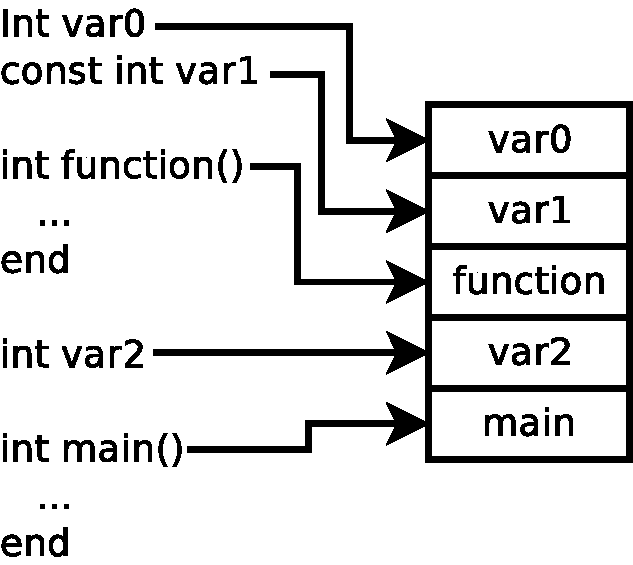
\includegraphics[width=0.33\textwidth]{images/Diagram1.pdf}
  \caption{Tablas de nombres globales}
  \label{fig:part2}
\end{figure}

Posteriormente tendremos una tabla de símbolos local que se creará en la entrada a una función y se eliminará al salir de la misma. En ella se contienen los parámetros de la función y las diferentes variables de la misma. El funcionamiento de la tabla de símbolos local puede verse en la \emph{figura} \ref{fig:part1}\subref{fig:1}, se puede comprobar como existe una tabla de símbolos para cada función.

\begin{figure}[H]
  \centering
  \subfloat[][Tabla de nombres locales]{\label{fig:1}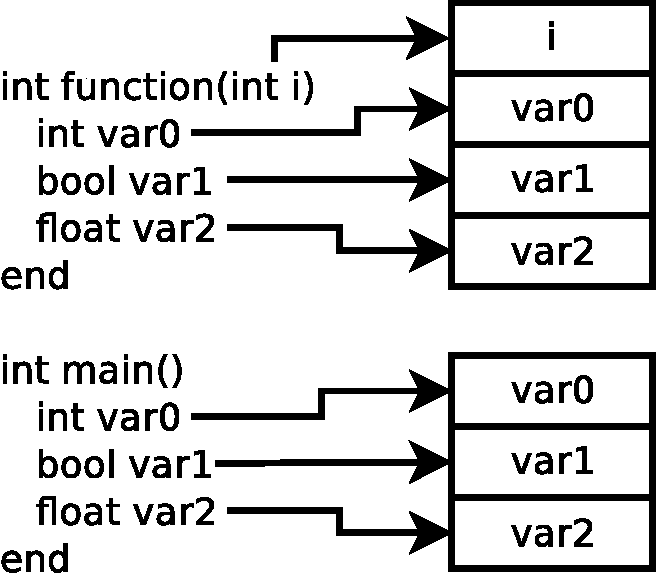
\includegraphics[width=0.33\textwidth]{images/Diagram2.pdf}}
  \hspace{11mm}
  \subfloat[][Tabla global de nombres locales]{\label{fig:2}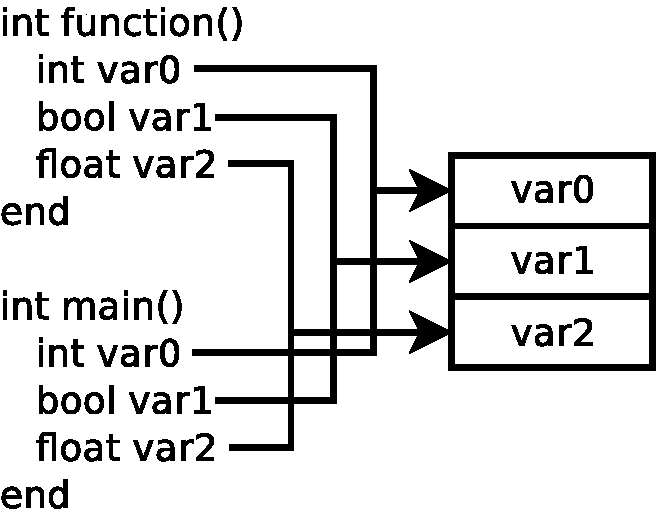
\includegraphics[width=0.33\textwidth]{images/Diagram3.pdf}}
  \caption{Tablas de nombres locales}
  \label{fig:part1}
\end{figure}

Finalmente, como cada símbolo local desaparece al finalizar la función y eliminarse la tabla, es importante mantener un registro de los nombres locales para evitar colisiones con símbolos globales, ello se debe a que hemos definido que no pueden existir símbolos locales y globales con el mismo nombre Para este tratamiento existe una tabla de nombres global de símbolos locales que contiene únicamente los nombres de las variables locales existentes, no habrá nombres repetidos puesto que si ya existe un nombre no repetiremos la inserción.Cuando se intente crear una variable global se hará una búsqueda en esta tabla para comprobar que no hay una colisión de nombres. Podemos ver el comportamiento de esta tabla en la \emph{figura} \ref{fig:part1} \subref{fig:1}

\begin{figure}[H]
  \centering
  \subfloat[][Error en la duplicación de nombres en varios ámbitos]{\label{fig:4}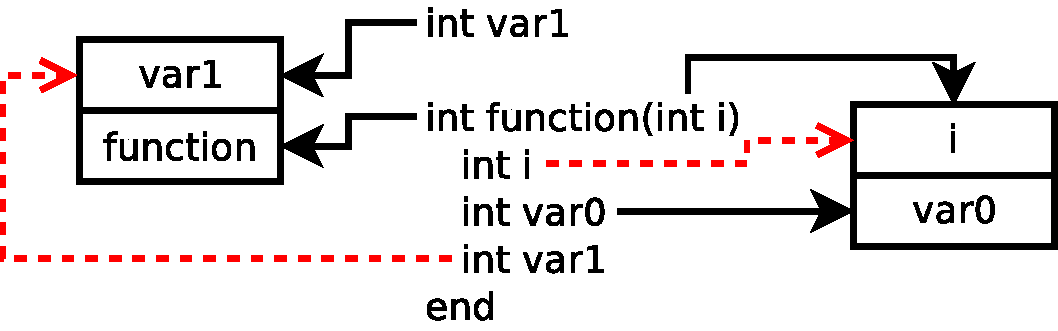
\includegraphics[width=0.5\textwidth]{images/Diagram5.pdf}}
  \hspace{11mm}
  \subfloat[][Duplicación de nombres locales]{\label{fig:3}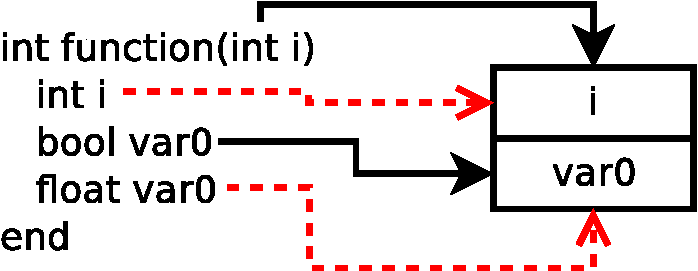
\includegraphics[width=0.4\textwidth]{images/Diagram6.pdf}}
  \caption{Errores en creación de nombres}
  \label{fig:part3}
\end{figure}

Ejemplos de colisiones pueden verse en la \emph{figura} \ref{fig:part3}. En la \emph{figura} \ref{fig:part3}\subref{fig:4} puede verse una colisión entre una variable local con una variable global ya existente y la colisión de una variable local con un parámetro del mismo nombre. En la \emph{figura} \ref{fig:part3}\subref{fig:3} puede verse una colisión de nombres locales, tanto de parámetros como de variables.

%\begin{figure}[H]
%  \centering
%	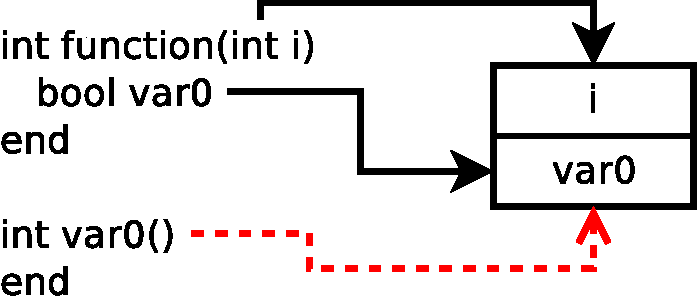
\includegraphics[width=0.4\textwidth]{images/Diagram7.pdf}
%  \caption{Tabla global de nombres locales}
%  \label{fig:part4}
%\end{figure}
\begin{figure}[H]
  \centering
  \subfloat[][Tabla global de nombres locales]{\label{fig:5}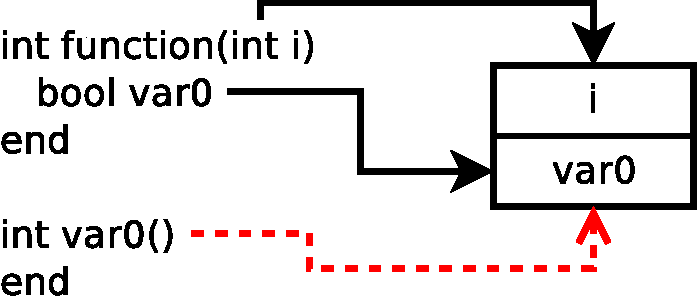
\includegraphics[width=0.4\textwidth]{images/Diagram7.pdf}}
  \hspace{11mm}
  \subfloat[][Parámetros de función]{\label{fig:6}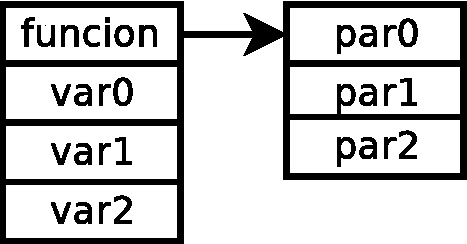
\includegraphics[width=0.33\textwidth]{images/Diagram8.pdf}}
  \caption{Errores en creación de nombres}
  \label{fig:part4}
\end{figure}
En la \emph{figura} \ref{fig:part4}\subref{fig:5} puede verse una colisión de un nombre global con un nombre local en la tabla global de nombres locales. Aunque el nombre global esté definido por debajo del global, se ha definido que no se pueden repetir nombres, es por ello que la tabla global de nombres locales es necesaria. 

En la \emph{figura} \ref{fig:part4}\subref{fig:6} puede verse la forma en que se almacenan los parámetros de una función. Se utilizará el campo parámetros de la estructura de información y cada parámetro contendrá al siguiente mediante el mismo puntero. De este modo se convierte en una lista de parámetros de la función.

La creación de símbolos para la inserción en la tabla correspondiente se realizará mediante una función específica. Esto permitirá ahorrar el trabajo del reservado de memoria e inicialización de cada campo. La función en sí es realmente simple y realiza una tarea igual de simple, pero debido a que estas acciones se repiten en numerosas ocasiones en el código se reduce mucho trabajo y muchas líneas de código:

\begin{lstlisting}
symbol_info *
create_symbol(	enum class clase,
								enum type tipo,
								enum boolean vector,
								int tam,
								enum boolean constant,
								enum boolean init,
								symbol_info *parametros)
\end{lstlisting}

Las tablas de símbolos globales se crearán en el inicio del programa. Las tablas de símbolos locales se crearán y destruirán a medida que se va entrando y saliendo de funciones. Para esta tarea se dispone de dos funciones que se encargarán de generar y destruir las tablas de símbolos locales, además inicializarán unas variables que determinarán que nos encontramos en un ámbito global o local:

\begin{lstlisting}
void int_function();
void out_function();
\end{lstlisting}

La inserción de nuevos símbolos se realiza mediante una función que se encargará de comprobar el ámbito en el que nos encontramos y decidir si el símbolo ha de insertarse en una tabla global o en una tabla local. En caso de tener que insertarse en una tabla global realizará la comprobación en la tabla global de símbolos locales. En caso de que el símbolo ya esté creado se lanzará un mensaje de error y se incrementará el contador de errores y se continuará con el análisis. La función será la siguiente:

\begin{lstlisting}
void st_new(char *name, symbol_info *info);
\end{lstlisting}

La búsqueda de símbolos se realizará de nuevo en el ámbito correspondiente, mediante una función que retornará el objeto de información de símbolo para su uso en el análisis:

\begin{lstlisting}
symbol_info *st_find(char *name);
\end{lstlisting}

Finalmente, existirá una función para destruir las tablas, los parámetros de los símbolos que sean funciones, y toda la memoria reservada en la creación de las tablas de símbolos. Esta función no eliminará tablas locales ya que estas se considerarán eliminadas llegadas a este punto:

\begin{lstlisting}
void st_destroy();
\end{lstlisting}

Entrelazando este código con la gramática mediante la introducción de código entre llaves se puede conseguir un análisis semántico con comprobación de los símbolos mediante tablas de símbolos. Además, mediante la información almacenada para cada símbolo en su estructura correspondiente se abre una puerta para un análisis semántico más potente.

\subsection{Comprobaciones semánticas}

Las comprobaciones semánticas permitirán definir si la forma en que interactúan los diferentes componentes es la correcta. Para ello se hará uso de información almacenada en las tablas de símbolos y de información que \textit{bison} nos permite transmitir entre reglas. Este mecanismo consiste en asignarle un tipo a cada regla, de forma que cuando se reduzcan, la regla que la contiene puede obtener información de la regla reducida. En consecuencia, aparecen nuevas variables a utilizar en el código de \textit{C}:

\begin{itemize}
	\item $\$\$$: nos permite asignarle un valor a la regla actual.
	\item $\$n$: dónde $n$ es un número entero que determina a que elemento de la regla nos estamos refiriendo y su contenido será el que se le asigne en dicha regla a $\$\$$ del tipo que se haya definido para dicha regla.
\end{itemize}

En nuestro caso, como hemos definido un tipo especial que contiene información, utilizaremos este tipo para algunas de las reglas ya que será necesario para que las reglas que están por encima puedan realizar ciertas comprobaciones:

\begin{lstlisting}
%type <info> ident decl_var_sim decl_funct_par_list 
%type <info> decl_funct_par funcall_pars decl_coma_list variable
\end{lstlisting}

Por otro lado, existen otras reglas para las que únicamente nos interesa su tipo, en estos casos devolveremos un entero que se corresponderá con el tipo de datos asociado en el código o en los tokens:
\begin{lstlisting}
%type <entero> type constant funcall expr_sec integer_const
%type <entero> expr_asig expression init_const atom
\end{lstlisting}

Los tipos de datos que devolverán las reglas anteriores están claramente definidos de forma ordinal para que algunos de los chequeos se puedan realizar con operaciones de comparación:

\begin{lstlisting}
enum type {T_VOID = -1, T_BOOL = 0, T_CHAR = 1, T_INT = 2, T_FLOAT = 3, T_STRING = 4};
\end{lstlisting}

Finalmente, la regla de nuevo identificador retornará únicamente una ristra conteniendo el nombre real del identificador. Esta regla y el resto de la información de la declaración de variables o de función servirá para insertar el símbolo en la tabla correspondiente con la información necesaria:

\begin{lstlisting}
%type <string> ident_new
\end{lstlisting}

Al finalizar todo el proceso de análisis semántico, se realizará una última comprobación en la tabla de símbolos en busca de la función \textit{main}. Si esta no existiera o estuviera mal definida, se lanzaría un error semántico y no se procedería con el proceso de compilación.

\subsubsection{Comprobaciones en la declaración de variables}

Cuando se declaran variables, se realizan una serie de comprobaciones en función de la forma en que esta es inicializada. Para empezar se comprueba que la variable no se ha declarado de tipo \textit{void}, lo cual sólo se permite en funciones que no retornan nada. El tipo \textit{void} devuelve un valor entero ordenado según nuestra conveniencia, \textit{void} es siempre menor que cero:

\begin{lstlisting}
	:	type ident_new 
		{
			if($1 < 0){
				printf("Line %d : variables can't be declared void\n",numline);
				numerrors++;
			} else {
			...
\end{lstlisting}

Puede observarse que el formato de errores el mismo que en el de los errores sintácticos de la función \textit{yyerror}. En principio el hecho de no usar la función \textit{yyerror} para mostrar estos errores consistía en la posibilidad de ofrecer errores más completos como en el caso de poder mostrar el nombre de una variable indefinida o duplicada.

El siguiente control consiste en comprobar, para variables con inicialización, que la inicialización es compatible. Es decir, se comprobará que no se intente inicializar una variable entera con una constante flotante, puesto que no son compatibles:
\begin{lstlisting}
	|	type ident_new '=' init_const 
		{
			...
			} else {
				if($4 == T_FLOAT && $1 < $4){
					printf("Line %d : type error in initialization\n",numline);
					numerrors++;
				} else {
			...
\end{lstlisting}

Posteriormente vendrán las comprobaciones de vectores. Comenzaremos con la comprobación de vectores de caracteres, con ristras como inicialización. Para empezar, si la inicialización es una ristra, el tipo del vector únicamente puede ser carácter. Posteriormente se comprobará que el tamaño de la ristra corresponderá con el tamaño de la constante entera que se ha utilizado para inicializar el tamaño del vector:

\begin{lstlisting}
	|	type ident_new '[' C_INT ']' '=' C_STRING  
		{
			if($1 != T_CHAR){
				printf("Line %d : strings have to be declared char\n",numline);
				numerrors++;
			} else {
				if($4 != string_size(yylval.string)){
					printf("Line %d : string initialization size error\n",numline);
					numerrors++;
				} else {
				...
\end{lstlisting}

Con respecto a los vectores inicializados mediante el vector de inicialización explicado anteriormente, es necesario explicar antes un elemento que contendrá la lista de valores de este vector. Se utilizará una estructura \textit{symbol\_info} para almacenar la información de esta regla, en el campo de tipo contendrá el mayor tipo de la lista y en el campo de tamaño contendrá el número de elementos del vector de inicialización:

\begin{lstlisting}
decl_coma_list				:	init_const ',' decl_coma_list 
												{
													...
													$3->tipo = ($1 > $3->tipo ? $1 : $3->tipo);
													$3->tam += 1;
													$$ = $3;
												}
											|	init_const 
												{
													$$ = create_symbol(VARIABLE, $1, NO, 1, NO, NO, NULL);
												}
\end{lstlisting}

Una vez volvemos a la declaración del vector, disponemos de la información de la declaración, sumada a la información del vector de inicialización. Sumada a las comprobaciones anteriormente descritas, comprobaremos que el vector de inicialización no devuelva una estructura nula, en realidad esto no puede suceder porque el sintáctico encontraría un error en este punto, pero como no todos los errores se tratan se ha añadido esta comprobación. Lo siguiente que hará será comprobar que la constante de tamaño del vector no sea menor o igual a cero, debido a la naturaleza de las constantes como elementos léxicos, menor que cero nunca será, pero sí puede ser igual a cero. Finalmente, el último añadido será la comprobación del tamaño del vector mediante la constante proporcionada por el programador y el número de elementos del vector de inicialización.

\begin{lstlisting}
	|	type ident_new '[' C_INT ']' '=' '[' decl_coma_list ']' 
		{
			if($1 < 0){
				printf("Line %d : variables can't be declared void\n",numline);
				numerrors++;
			} else {
				if($8 == NULL){
					printf("Line %d : vector initialization size error\n",numline);
					numerrors++;
				} else {
					if($4 <= 0){
						printf("Line %d : vector size error\n",numline);
						numerrors++;
					}
					
					if($4 != $8->tam){
						printf("Line %d : vector initialization size error\n",numline);
						numerrors++;
					}
					
					if($8->tipo == T_FLOAT && $1 < $8->tipo){
						printf("Line %d : type error in initialization\n",numline);
						numerrors++;
					} else {
\end{lstlisting}

No se ha mostrado ni se ha comentado, pero a medida que se comprueba que cada declaración es semánticamente correcta, se va haciendo la correspondiente inserción en la tabla de símbolos correspondiente. 
\subsubsection{Comprobaciones en los saltos}

Las comprobaciones en los saltos impedirán que se utilicen sentencias \textit{break} y \textit{continue} fuera de bucles ya que esto carecería de sentido. Esto se podrá realizar ya que cada vez que se entra en un bucle, se inicializará una variable para mantener este control:

\begin{lstlisting}
stmnt_jump						:	CONTINUE 
												{
													if(iteration == 0){
														printf("Line %d : continue statement shouldn't be here\n",numline);
														numerrors++;
													} 
												} '\n'
											|	BREAK 
												{
													if(iteration == 0){
														printf("Line %d : break statement shouldn't be here\n",numline);
														numerrors++;
													}
\end{lstlisting}
\subsubsection{Comprobaciones en las llamadas a funciones}

Cuando se realizan llamadas a funciones, es conveniente comprobar que los parámetros insertados son los correctos. Para ello, cuando se define una función se almacenan en su estructura de símbolo información adicional correspondiente a cada uno de los parámetros de dicha función. El símbolo de la función se ha de almacenar en la tabla de símbolos global, sin embargo, los parámetros se deben insertar en la local a la función, es por ello que se realiza un reajuste del nivel en el que nos encontramos:

\begin{lstlisting}
	type ident_new '(' decl_funct_par ')' 
												{
													int val = 0;
													level = 0; 
													symbol_info *info = $4;
													while(info){
														info = info->parametros;
														val++;
													}
													st_new($2, create_symbol(FUNCTION, $1, NO, val, NO, NO, $4)); 
													level = 1;
												} 
\end{lstlisting}

A medida que se recorren cada uno de los parámetros de la función, se va generando una lista de elementos de información de símbolo, cuyo siguiente elemento se hallará en el puntero a parámetros y cuyo final se encontrará cuando se alcance un puntero a nulo:

\begin{lstlisting}
decl_funct_par				:	{in_function();} 
												decl_funct_par_list
												{$$ = $2;}

decl_funct_par_list		:	decl_var_sim ',' decl_funct_par_list
												{
													...
													$1->parametros = $3;
													$$ = $1;
												}
												
											|	decl_var_sim
												{$$ = $1;}
\end{lstlisting}

A medida que se recorren los parámetros, se van generando nuevos nombres en la tabla de símbolos local de la función. Del mismo modo se realiza una comprobación de que el tipo de los parámetros no ha sido definido \textit{void}, puesto que ya dijimos que este tipo sólo podía darse como retorno de función:
\begin{lstlisting}
decl_var_sim					:	type ident_new 
												{
													if($1 < 0){
														printf("Line %d : variables can't be declared void\n",numline);
														numerrors++;
													} else {
														st_new($2, create_symbol(VARIABLE, $1, NO, 0, NO, NO, NULL));
														$$ = create_symbol(VARIABLE, $1, NO, 0, NO, NO, NULL);
														...
													}
												}
												
											|	type ident_new '[' ']' 
												{
													if($1 < 0){
														printf("Line %d : variables can't be declared void\n",numline);
														numerrors++;
													} else {
														st_new($2, create_symbol(VARIABLE, $1, YES, 0, NO, NO, NULL));
														$$ = create_symbol(VARIABLE, $1, YES, 0, NO, NO, NULL);
														...
													}
												}
												
\end{lstlisting}


Una vez tenemos el nombre de la función, obtenemos el símbolo de la tabla \textit{hash} y realizamos las comprobaciones pertinentes. En primer lugar, si la función está definida para no tener parámetros, al encontrarnos en la regla para funciones con parámetros, lanzaremos un error. En caso de que no sea así, se realizará una comprobación de cada uno de los parámetros de la llamada y de la especificación. Esto se podrá realizar porque el elemento \textit{funcall\_pars} es una lista de parámetros del mismo tipo que la contenida en la estructura de símbolo de la función:

\begin{lstlisting}
	:	ident '(' funcall_pars ')'
		{
			if($1 != NULL){
				if($1->parametros != NULL){
					int i = 0;
					symbol_info *aux;
					symbol_info *param_chk = $3;
					symbol_info *param_real = $1->parametros;

					while(param_chk != NULL && param_real != NULL){
						i++;
						if(param_chk->tipo > param_real->tipo){
							
							if(!(param_chk->tipo == T_STRING && 
								 param_real->tipo == T_CHAR && 
								 param_real->vector == YES
								 )){
								printf("Line %d : function parameter %d type is wrong\n", numline, i);
								numerrors++;
							}
						}
						param_chk = param_chk->parametros;
						param_real = param_real->parametros;
					}

					if(param_chk != NULL || param_real != NULL){
						printf("Line %d : wrong number of parameters\n", numline);
						numerrors++;
					}

					param_chk = $3;
					while(param_chk != NULL){
						aux = param_chk;
						param_chk = param_chk->parametros;
						free(aux);
					}
					...
					$$ = $1->tipo;
				} else {
					printf("Line %d : function does not have parameters\n",numline  );
					numerrors++;
				}
			}
		}
\end{lstlisting}
Finalmente, se comprobará, si el número de parámetros es el mismo volver a lanzar un error en caso de que no sea así. En las llamadas a funciones sin parámetros únicamente se comprobará si la función requiere parámetros, en caso afirmativo se lanzará un error puesto que no es la regla adecuada:

\begin{lstlisting}
	|	ident '(' ')' 
		{
			if($1 != NULL){
				if($1->parametros == NULL){
					$$ = $1->tipo;
					...
				} else {
					printf("Line %d : function needs parameters\n",numline  );
					numerrors++;
				}
			}
		}
	;
\end{lstlisting}
\subsubsection{Comprobaciones en el uso de variables}
La comprobación que se realiza en el uso de las variables será en aquellas que se traten como vectores sin serlo. Esto no tiene ningún sentido real ya que un vector consistirá en un bloque de datos, mientras que una variable será un único dato:

\begin{lstlisting}
	|	ident '[' expr_sec ']'
	{
		if($1 != NULL){
			if($1->vector == 0){
				printf("Line %d : vector usage error\n",numline  );
				numerrors++;
			}
			...
		}
	}
	;
\end{lstlisting}
\subsubsection{Comprobaciones en las expresiones}

La comprobación en las expresiones de asignación permitirá evitar que una operación de asignación se pueda realizar sobre una variable definida con el modificador de constante. Además impedirá que tipos no enteros se asignen a tipos enteros o que tipos vectoriales (ristras) se asignen a los demás tipos:

\begin{lstlisting}
	:	variable '=' expr_sec 
		{
			if($1 != NULL){
				if($1->constant == YES){
					printf("Line %d : constant variable can't be modified\n",numline-1);
					numerrors++;
				}
				if(($3 == T_FLOAT && $1->tipo < $3) || 
					 ($1->tipo == T_FLOAT && $1->tipo < $3) ||
					 ($1->tipo  <= T_INT   &&    T_INT < $3) ||  
					 ($3 < 0))
				{
					printf("Line %d : type error in assignment\n",numline-1);
					numerrors++;
				} 
				$$ = $1->tipo;
			}
\end{lstlisting}

Finalmente y debido a que disponemos de aritmética en punto flotante desde el punto de vista sintáctico y semántico, existirán algunos operadores que únicamente puedan disponer de operandos enteros. Ellos serán principalmente las operaciones booleanas (and, or, xor), los desplazamientos y el módulo:
\begin{lstlisting}
		if($1 > T_INT || $3 > T_INT ){
			printf("Line %d : ^ is an integer operation\n",numline-1);
			numerrors++;
		} 
\end{lstlisting}


\subsection{Generación del AST}
La generación del árbol sintáctico abstracto no es una tarea específica de la asignatura, pero ha sido realizada debido a que se ha querido ir un poco más allá en el aprendizaje sobre el desarrollo de compiladores. El árbol sintáctico abstracto es una estructura recursiva, extremadamente elegante, que permite realizar un tratamiento del código mucho más directo y con toda la información necesaria. 

Cada nodo del árbol representará a un elemento del código, por ejemplo, puede existir un nodo que represente a un bucle, otro que represente una expresión, etc. En nuestro caso, para la diferenciación de cada uno de estos elementos del código hemos definido una serie de macros en forma de \textit{enum}:
\begin{lstlisting}
enum ast_type {
	AST_PROG, AST_FUN, AST_VAR, 
	
	AST_FOR, AST_WHILE, 
	AST_IF, AST_ELSIF, AST_ELSE,
	AST_SWITCH, AST_CASE, AST_DEFAULT,
	
	AST_BREAK, AST_CONT, AST_RET,
	
	AST_FUNCALL, AST_IDENT, AST_CONST, AST_EXPR,
	
	AST_OUT, AST_IN, 
	
	AST_B_MUL, AST_B_DIV, AST_B_MOD, AST_B_SUM, 
	AST_B_MIN, AST_B_SRGT, AST_B_SLFT, AST_B_GEQ,
	AST_B_SEQ, AST_B_GT, AST_B_ST, AST_B_NEQ, AST_B_EQ,
	AST_B_ORB, AST_B_ANDB, AST_B_XOR, AST_B_OR,
	AST_B_AND, AST_B_ASIG,
	 
	AST_U_POS, AST_U_MIN, AST_U_NEG, AST_U_NEGB,
};
\end{lstlisting}

Además de ello, se han definido una serie de subtipos, que consistirán en el tipo de datos del elemento. En general esto se utilizará para las llamadas a funciones, identificadores, expresiones, constantes y variables. De este modo se podrá realizar una traducción del código más personalizada según el tipo de dato que corresponda:

\begin{lstlisting}
enum ast_subtype {AST_VOID = -1, AST_BOOL = 0, AST_CHAR = 1, 
									AST_INT = 2, AST_FLOAT = 3, AST_STRING = 4};
\end{lstlisting}


La definición de la estructura del árbol sintáctico no es una tarea estándar, y nosotros hemos definido nuestro propio árbol en el que cada nodo tiene la siguiente configuración:
\begin{itemize}
	\item \textbf{Type:} consiste en el tipo de elemento del código en el que nos encontramos.
	\item \textbf{Subtype:} consiste en el tipo de datos del elemento.
	\item \textbf{String:} será un puntero a una ristra de caracteres que se utilizará para almacenar información literal cuando sea necesario.
	\item \textbf{Integer:} permitirá almacenar un entero, ya sea para constantes o para alguna otra tarea.
	\item \textbf{Real:} del mismo modo, permitirá almacenar un número real, aunque únicamente para constantes.
	
	\item \textbf{Type\_info:} será un vector a punteros de tipo nodo de árbol \textit{ast}. Se utilizarán para definir elementos que sean propios del elemento actual, por ejemplo la condición de un \textit{if}.
	
	\item \textbf{Content:} será un puntero al inicio del bloque contenido por el elemento actual. No todos los elementos del código tienen bloques, sólo las estructuras y las funciones.
	
	\item \textbf{Sibling:} será un puntero al siguiente nodo en el mismo nivel de la jerarquía, por ejemplo estando en una función, sería un puntero a ota función.
	
\end{itemize}

A continuación se muestra el código correspondiente con lo explicado:
\begin{lstlisting}
struct ast_node_ {
	enum ast_type type;
	enum ast_subtype subtype;
	char *string;
	int integer;
	float real;

	struct ast_node_ **type_info;
	struct ast_node_ *content;
	struct ast_node_ *sibling;
};

typedef struct ast_node_ ast_node;
\end{lstlisting}


Para la creación de nodos dispondremos de una función predeterminada, ésta reservará la memoria necesaria e inicializará todos los campos mediante la información proporcionada por los parámetros de la función. Del mismo modo y al ser una estructura recursiva cuyo recorrido se realizará en función del tipo de nodo en que nos encontremos, tendremos una única función de destrucción del árbol:

\begin{lstlisting}
ast_node* 
ast_node_create(enum ast_type,
								enum ast_subtype,
								char *,
								int,
								float,
								ast_node **,
								ast_node *,
								ast_node *);
								
void ast_node_destroy(ast_node *);
\end{lstlisting}

La creación del árbol se realizará mediante código embebido en el análisis sintáctico y semántico. Este código será extremadamente simple y seguirá un proceso lógico:

\begin{enumerate}
\item Se creará el elemento en el que nos encontramos con la información que necesitamos y sacando tantos elementos de la pila como se requiera.
\item Se insertará el elemento en una pila específicamente creada para la generación del árbol.
\item Se subirá un nivel en el análisis por reducción, si nos encontramos en el estado final, se finalizará. Si por el contrario nos encontramos en un nodo intermedio, procederemos de nuevo a 1.
\end{enumerate}

Finalmente, este árbol será el retorno de la función de análisis léxico/sintáctico/semántico y se utilizará en última instancia para la generación de código. A continuación se explicará de forma rápida y mediante soporte gráfico la definición de cada uno de los nodos y como deben ser utilizados.

En el nivel más alto del árbol sintáctico tendremos el nodo correspondiente con el programa, se puede observar en la \emph{figura} \ref{fig:prog}. Este nodo contiene dos elementos de tipo principales, las funciones y las variables globales. La separación de ambas permite un tratamiento independiente de las mismas, de modo que se pueda mantener la coherencia en la generación de código.

\begin{figure}[H]
  \centering
  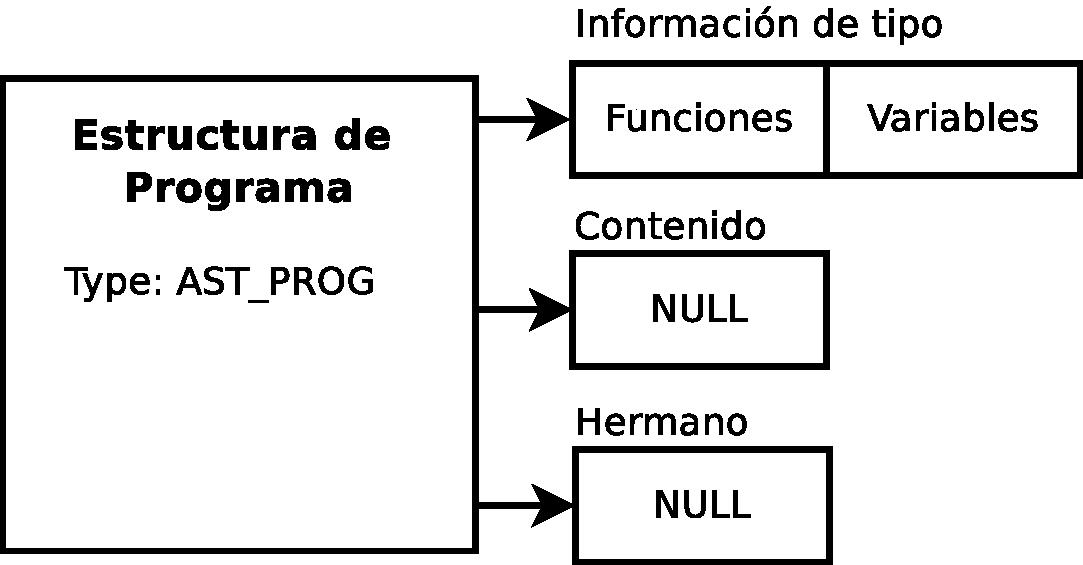
\includegraphics[width=0.40\textwidth]{images/ast_prog.pdf}
  \caption{Programa}
  \label{fig:prog}
\end{figure}

Posteriormente tendremos los nodos correspondientes con las variables (\emph{figura} \ref{fig:funvar}\subref{fig:astvar}) y las funciones (\emph{figura} \ref{fig:funvar}\subref{fig:astfun}). El nodo de variables se utiliza tanto para definir variables globales, como para definir variables y parámetros dentro de funciones (que irán debajo del correspondiente nodo de función). Contendrán, en algunos casos, en su información de tipo una constante de inicialización y en su puntero hermano contendrán la siguiente variable. Los nodos de función, en su información de tipo, contendrán un nodo para los parámetros, que consistirá en una lista de variables, y un nodo para las variables, que también será una lista. Además dispondrá de un bloque de código en el puntero de contenido y de posibles funciones en la misma jerarquía bajo el puntero de hermanos.
\begin{figure}[H]
  \centering
  \subfloat[][Nodo de declaración de función]{\label{fig:astfun}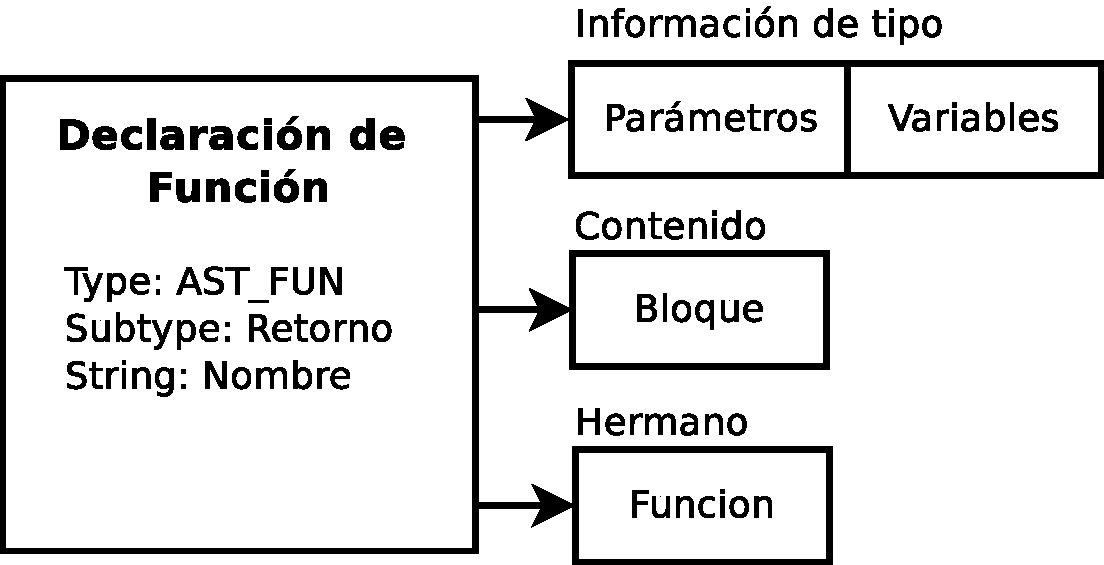
\includegraphics[width=0.40\textwidth]{images/ast_fun.pdf}}
  \hspace{11mm}
  \subfloat[][Nodo de declaración de variable]{\label{fig:astvar}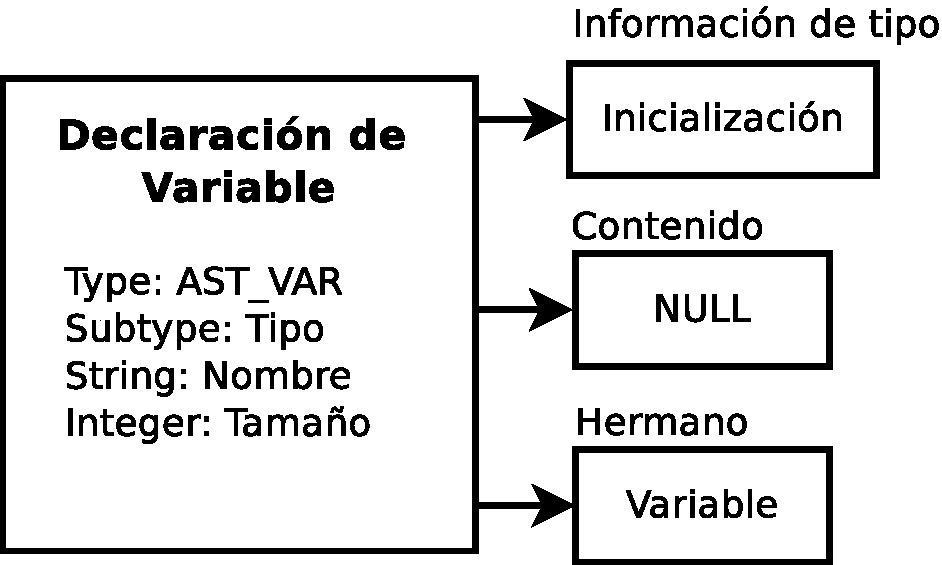
\includegraphics[width=0.33\textwidth]{images/ast_var.pdf}}
  \caption{Elementos globales}
  \label{fig:funvar}
\end{figure}

Dentro del nivel de bloques, tenemos los bucles. Existen dos posibles bucles, el \textit{for} y el \textit{while}. El bucle \textit{for} se puede ver en la \emph{figura} \ref{fig:bucles}\subref{fig:astfor}, como información de tipo contiene una serie de expresiones de inicialización de la variable, condición de salida y el paso del bucle. Al ser una estructura también contendrá un bloque. Finalmente, en el puntero a hermano podrá contener código de la misma jerarquía. La diferencia con el bucle \textit{while} (\emph{figura} \ref{fig:bucles}\subref{fig:astwhile}) será que en la información de tipo ésta sólo contendrá una expresión que será una condición de salida.
\begin{figure}[H]
  \centering
  \subfloat[][Nodo de bucle for]{\label{fig:astfor}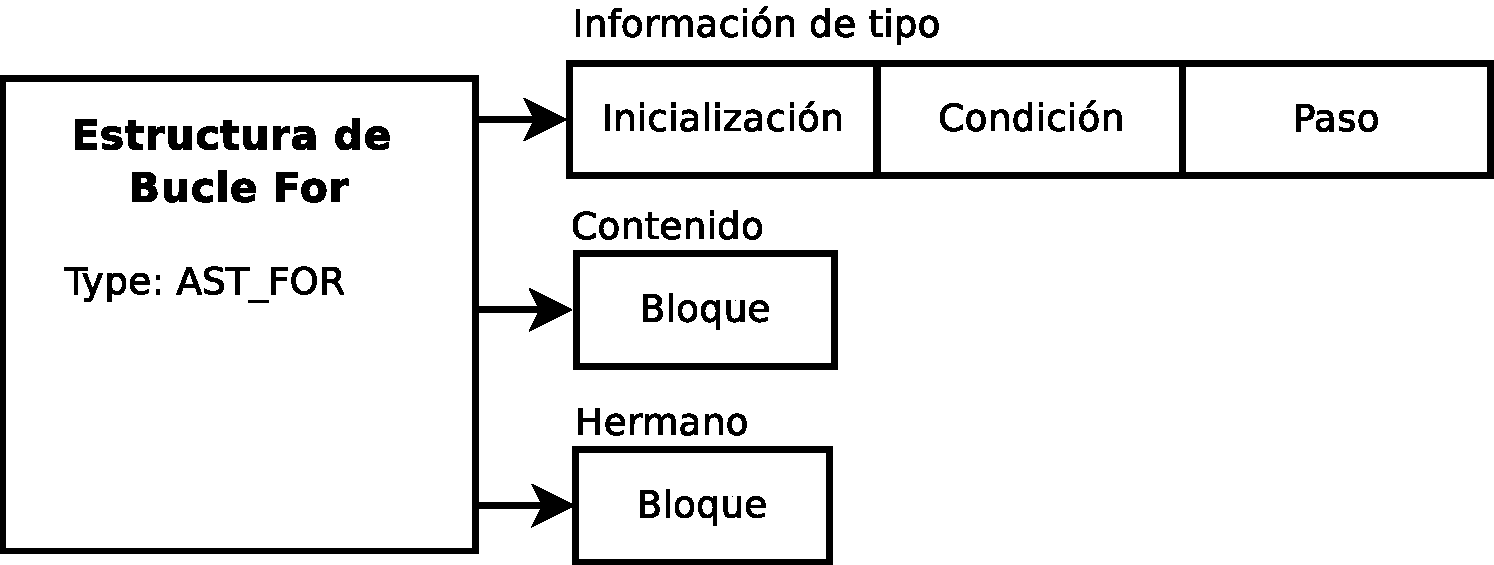
\includegraphics[width=0.53\textwidth]{images/ast_for.pdf}}
  \hspace{11mm}
  \subfloat[][Nodo de bucle while]{\label{fig:astwhile}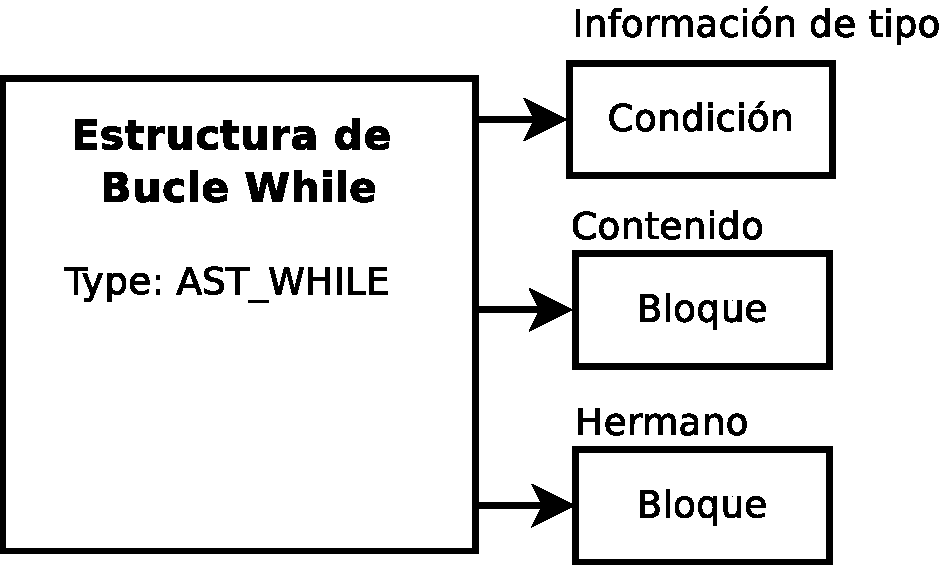
\includegraphics[width=0.33\textwidth]{images/ast_while.pdf}}
  \caption{Bucles}
  \label{fig:bucles}
\end{figure}

Como sentencias de selección tenemos el \textit{if} (\emph{figura} \ref{fig:sel1}\subref{fig:astif}), que contendrá como información de tipo una condición del \textit{if} y un puntero a los posibles \textit{elsif} y \textit{else} (\emph{figura} \ref{fig:sel2}\subref{fig:astelsif}\subref{fig:astelse}). Además contendrá un bloque ya que es una estructura y un puntero al código del mismo nivel de la jerarquía.
\begin{figure}[H]
  \centering
  \subfloat[][Nodo de selección if]{\label{fig:astif}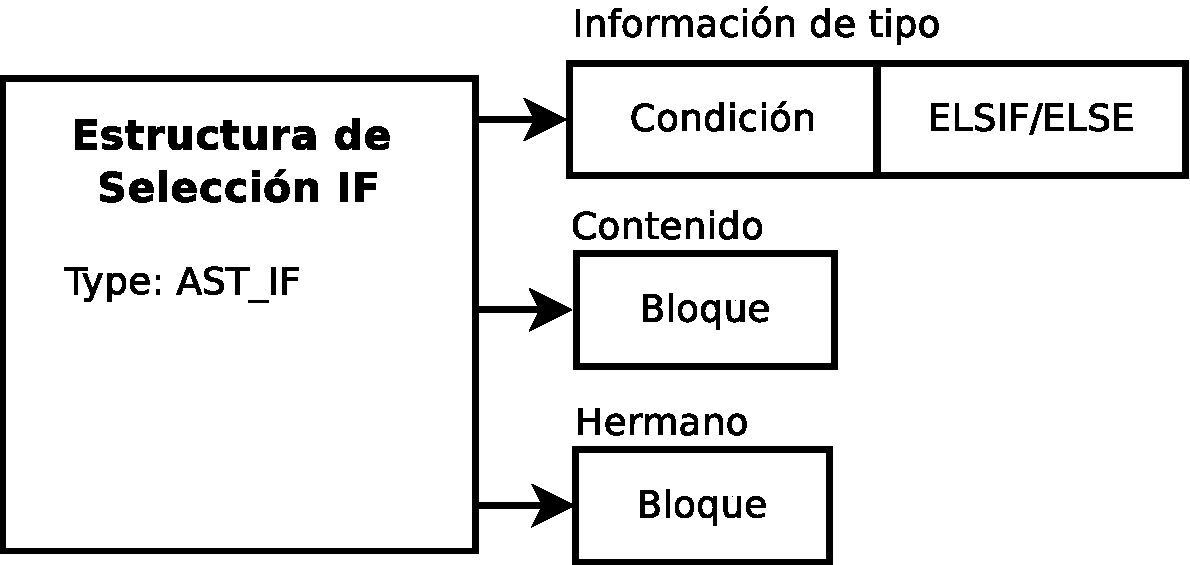
\includegraphics[width=0.42\textwidth]{images/ast_if.pdf}}
  \hspace{11mm}
  \subfloat[][Nodo de selección switch]{\label{fig:astswitch}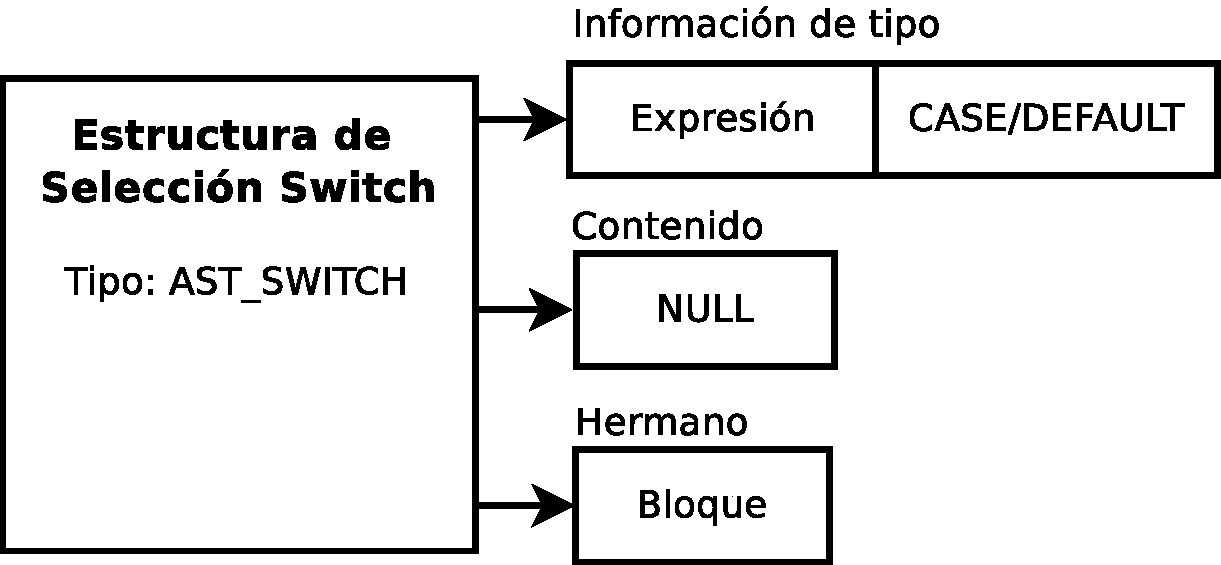
\includegraphics[width=0.42\textwidth]{images/ast_switch.pdf}}
  \caption{Sentencias de selección}
  \label{fig:sel1}
\end{figure}

También disponemos de la sentencia \textit{switch} (\emph{figura} \ref{fig:sel1}\subref{fig:astswitch}), que contendrá como información de tipo la expresión del \textit{switch} que será comparada con las constantes de los case y un puntero a los case y \textit{default} (\emph{figura} \ref{fig:sel3}\subref{fig:astcase}\subref{fig:astdefault}). No tendrá bloque ya que el contenido de esta estructura se dará en los case y si tendrá un puntero hacia el código de la misma jerarquía.
\begin{figure}[H]
  \centering
  \subfloat[][Nodo de selección elsif]{\label{fig:astelsif}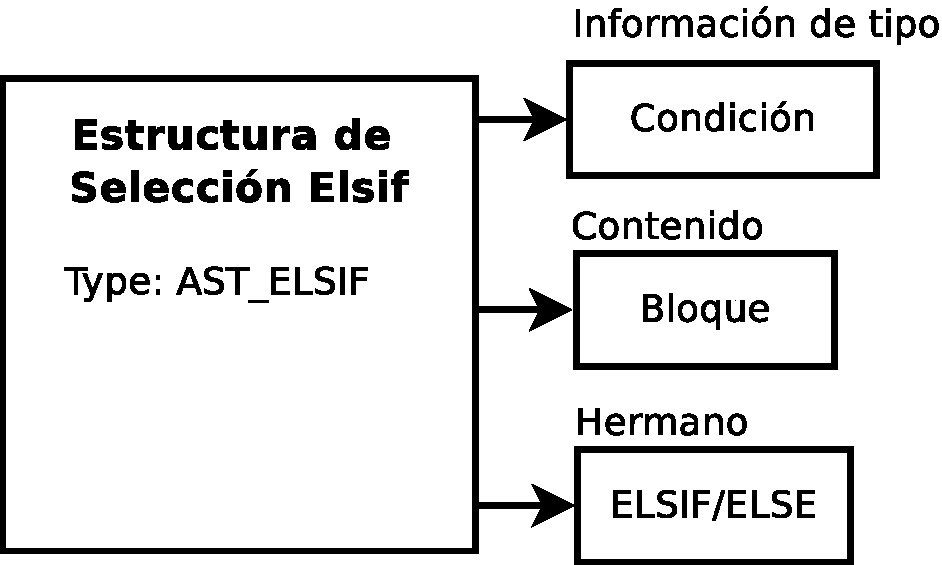
\includegraphics[width=0.33\textwidth]{images/ast_elsif.pdf}}
  \hspace{11mm}
  \subfloat[][Nodo de selección else]{\label{fig:astelse}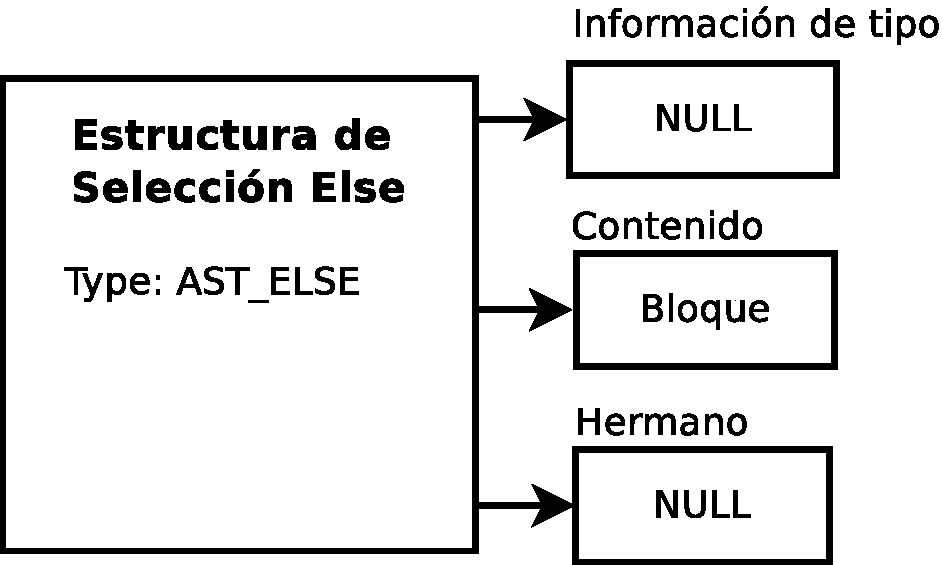
\includegraphics[width=0.33\textwidth]{images/ast_else.pdf}}
  \caption{Sentencias de selección}
  \label{fig:sel2}
\end{figure}

Las estructuras elsif (\emph{figura} \ref{fig:sel2}\subref{fig:astelse}) tendrán el mismo comportamiento que la sentencia \textit{if}, ello quiere decir que mediante una expresión decidirán si se ejecuta el bloque apuntado por contenido o se procede con la siguiente sentencia \textit{elsif} o \textit{else} apuntada por el puntero a hermano. Todo bloque de sentencias \textit{elsif} o \textit{else} puede contener múltiples \textit{elsif}, pero un único \textit{else}. Este \textit{else} (\emph{figura} \ref{fig:sel2}\subref{fig:astelse}) sólo contendrá un puntero al bloque de código que se ejecutará si se llega a este nodo.

En el caso de los \textit{switch}, el comportamiento de los case será similar, sólo que en vez de utilizarse una expresión, se comparará el resultado de la expresión del \textit{switch} con una constante contenida en el parámetro de información. En caso de coincidir, se ejecutará el código situado en el puntero al contenido de cada case, en caso contrario se pasará a la siguiente condición, que podrá ser un case o un \textit{default} (\emph{figura} \ref{fig:sel3}\subref{fig:astdefault}). En el caso del \textit{default}, sólo se ejecutará el código del bloque.
\begin{figure}[H]
  \centering
  \subfloat[][Nodo de selección case]{\label{fig:astcase}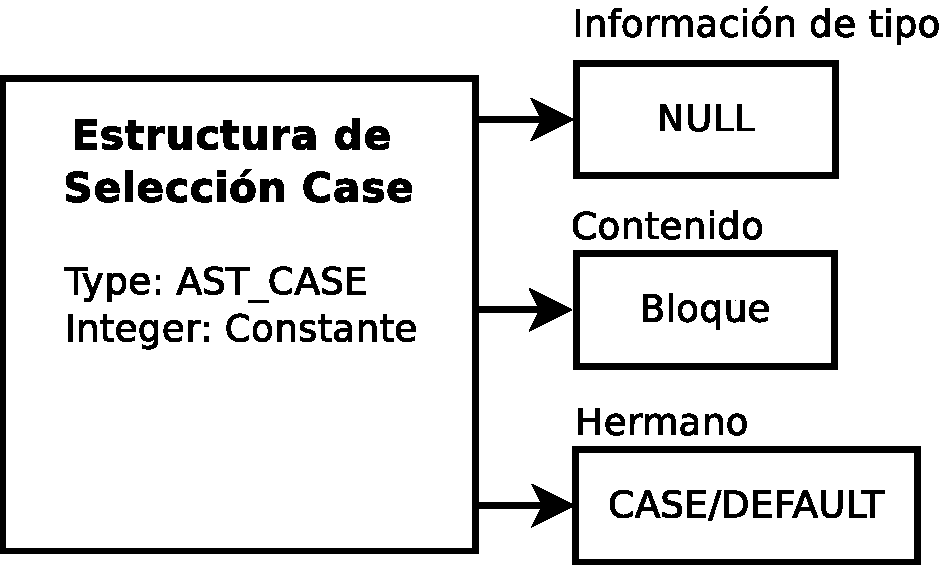
\includegraphics[width=0.33\textwidth]{images/ast_case.pdf}}
  \hspace{11mm}
  \subfloat[][Nodo de selección default]{\label{fig:astdefault}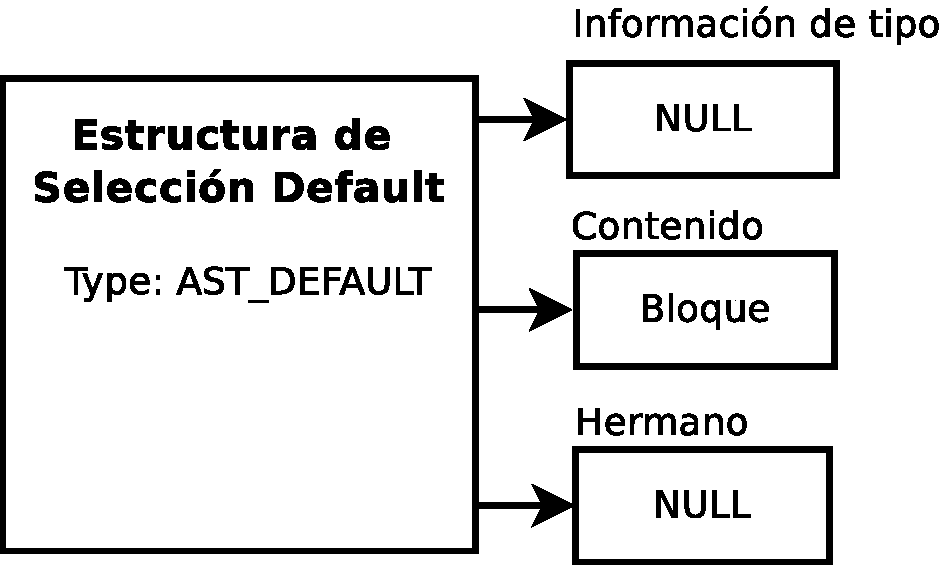
\includegraphics[width=0.33\textwidth]{images/ast_default.pdf}}
  \caption{Sentencias de selección}
  \label{fig:sel3}
\end{figure}

Los saltos (\emph{figura} \ref{fig:saltos}) son nodos extremadamente simples, no tienen ningún tipo de contenido y sólo tienen un puntero al código hermano de la misma jerarquía. Sin embargo, existe una excepción. En el caso de las sentencias \textit{return} (\emph{figura} \ref{fig:saltos}\subref{fig:astreturn}) podemos contener una expresión cuyo resultado será el valor de retorno de la función.
\begin{figure}[H]
  \centering
  \subfloat[][Nodo de salto break]{\label{fig:astbreak}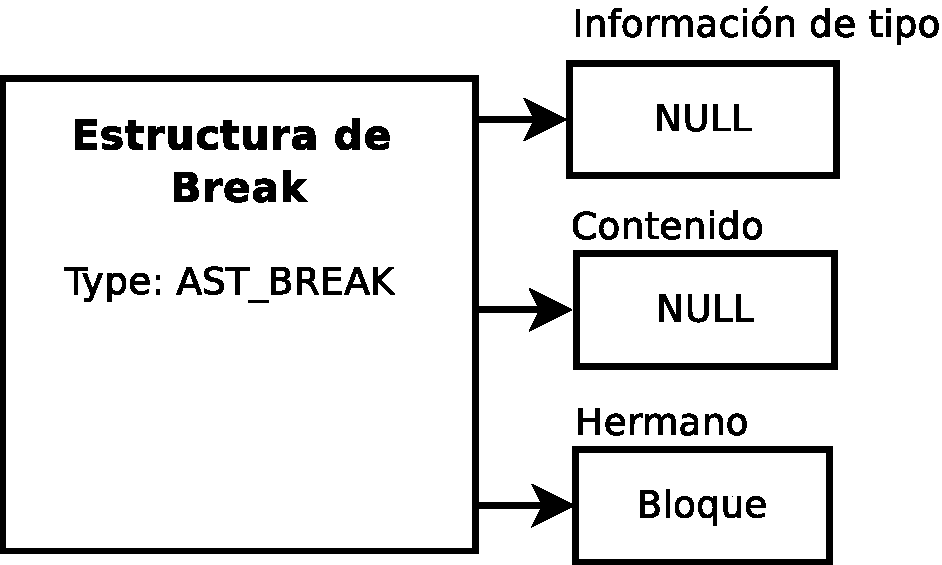
\includegraphics[width=0.33\textwidth]{images/ast_break.pdf}}
  \subfloat[][Nodo de salto continue]{\label{fig:astcontinue}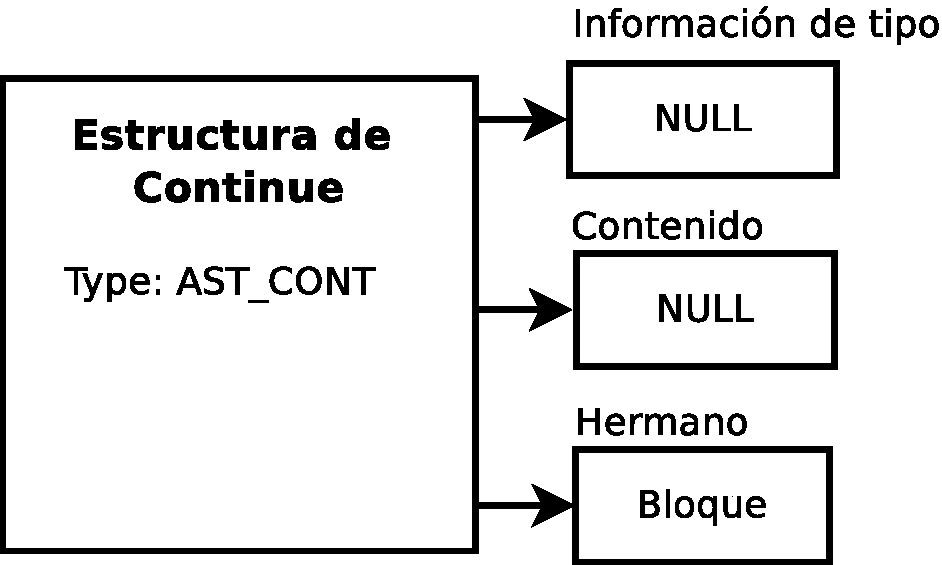
\includegraphics[width=0.33\textwidth]{images/ast_cont.pdf}}
  \subfloat[][Nodo de salto return]{\label{fig:astreturn}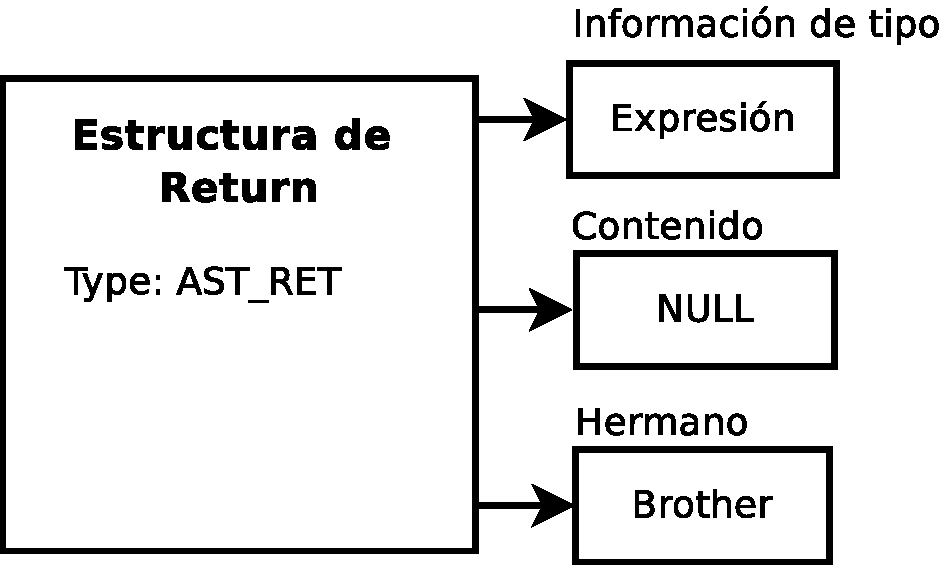
\includegraphics[width=0.33\textwidth]{images/ast_ret.pdf}}
  \caption{Saltos}
  \label{fig:saltos}
\end{figure}

El nodo de expresión (\emph{figura} \ref{fig:exprop}\subref{fig:astexpr})deforma ligeramente la estructura y resulta más propio de un árbol sintáctico concreto. Sin embargo, es una forma de mantener las expresiones encapsuladas. Contiene, en su puntero de contenido, lo que realmente será la expresión. Lo habitual será una expresión que utilice un operador binario un operador unario(\emph{figura} \ref{fig:exprop}\subref{fig:astuop}), pero puede contener elementos de más bajo nivel.
\begin{figure}[H]
  \centering
  \subfloat[][Nodo de expresión]{\label{fig:astexpr}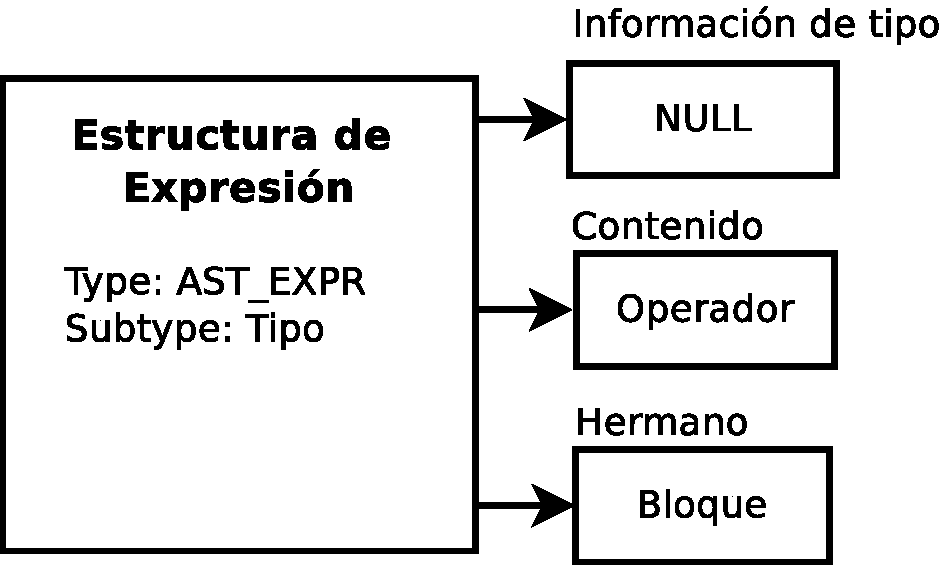
\includegraphics[width=0.33\textwidth]{images/ast_expr.pdf}}
  \hspace{11mm}
  \subfloat[][Nodo de operador unario]{\label{fig:astuop}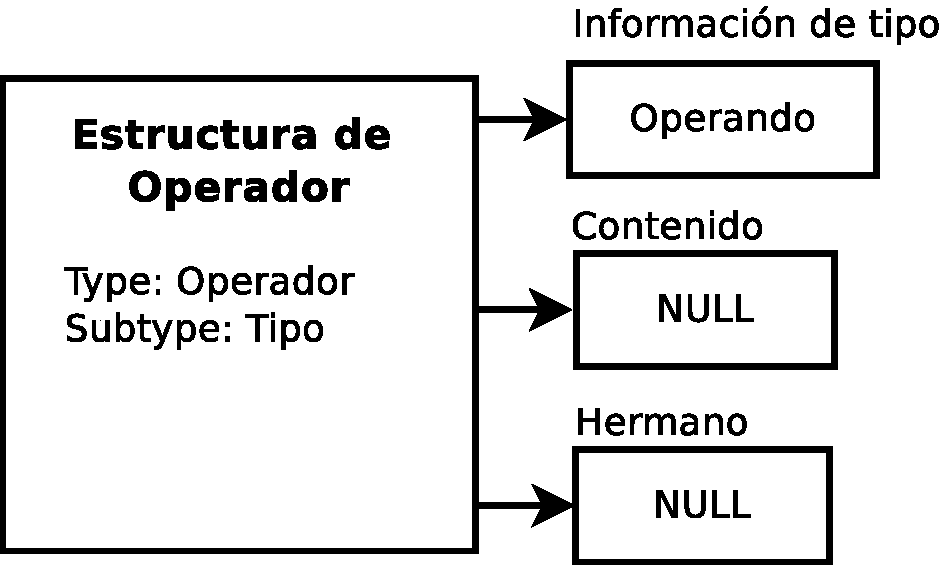
\includegraphics[width=0.33\textwidth]{images/ast_uop.pdf}}
  \caption{Expresiones y operadores}
  \label{fig:exprop}
\end{figure}

Los operadores binarios contendrán dos operandos en su información de tipo (en forma de lista). Los operadores unarios, como su propio nombre indica, contendrá únicamente un operando. Este operando puede ser un elemento de más bajo nivel, como un identificador o una constante, o un elemento del mismo nivel como otro operador.

Las estructuras de más bajo nivel en las expresiones (\emph{figura} \ref{fig:atom}) serán las constantes, los identificadores y las llamadas a funciones. Las primeras contendrán toda su información en los campos de las estructura del nodo, las segundas permitirán una expresión de que se esté intentando acceder a los elementos de un vector, y los terceros contendrán una lista de parámetros en su campo de información. Los parámetros serán, generalmente, expresiones.
\begin{figure}[H]
  \centering
  \subfloat[][Nodo de constante]{\label{fig:astconst}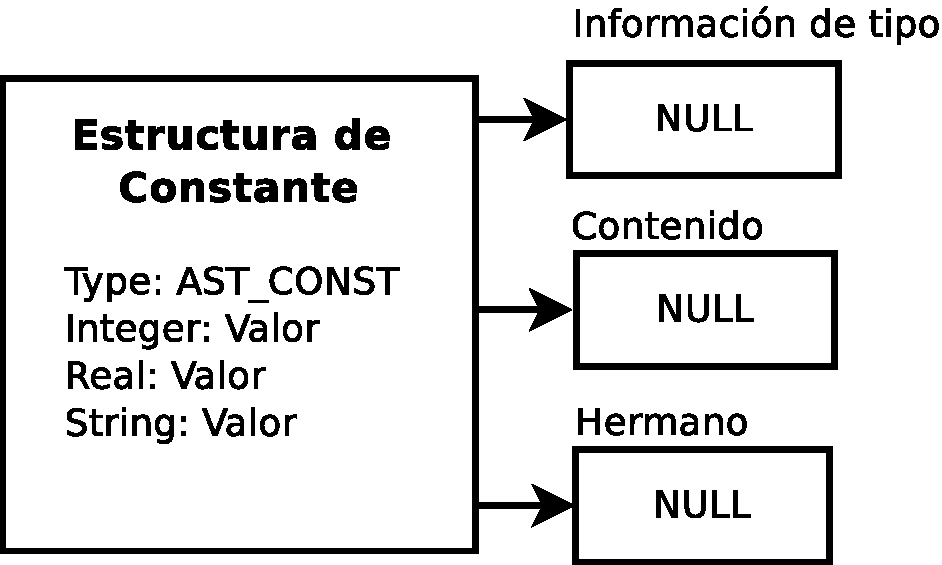
\includegraphics[width=0.33\textwidth]{images/ast_const.pdf}}
  \subfloat[][Nodo de identificador]{\label{fig:astident}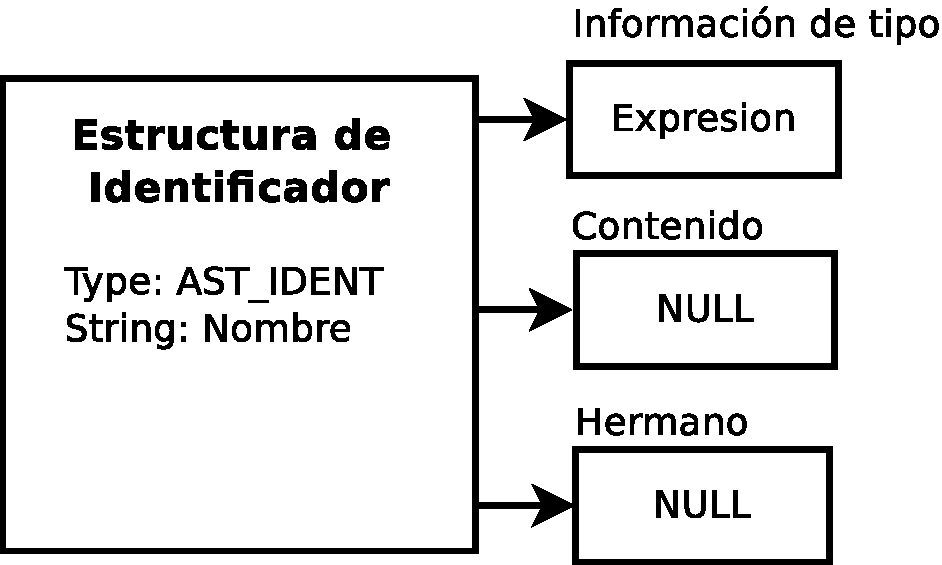
\includegraphics[width=0.33\textwidth]{images/ast_ident.pdf}}
  \subfloat[][Nodo de llamada a función]{\label{fig:astfuncall}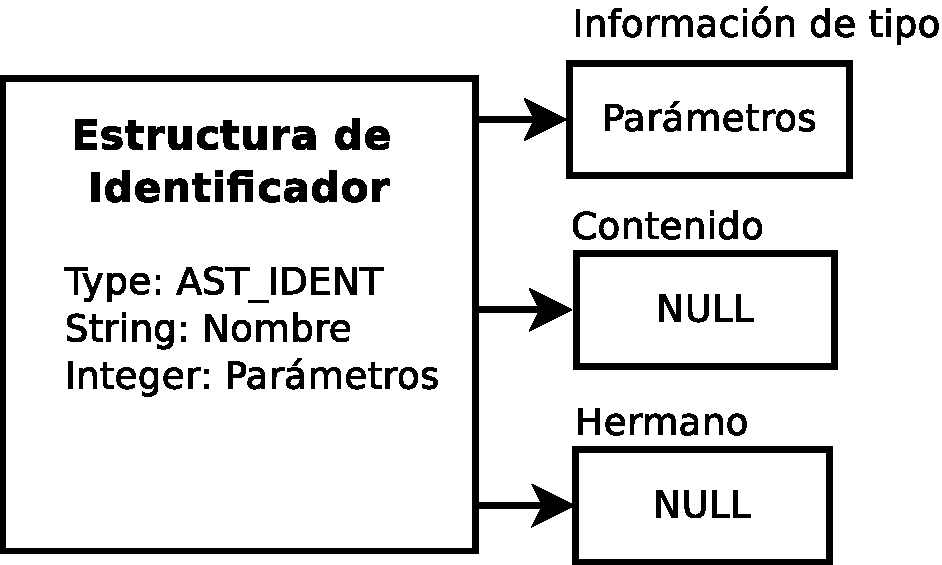
\includegraphics[width=0.33\textwidth]{images/ast_funcall.pdf}}
  \caption{Elementos atómicos}
  \label{fig:atom}
\end{figure}

Finalmente, tendremos los nodos correspondientes con las expresiones de entrada y salida (\emph{figura} \ref{fig:exprio}). La entrada (\emph{figura} \ref{fig:exprio}\subref{fig:exprin}) contendrá únicamente una variable (nodo identificador) en el cual almacenará el valor correspondiente al carácter leído de la entrada estándar. La salida (\emph{figura} \ref{fig:exprio}\subref{fig:exprout}) contendrá una lista de las variables  o constantes de salida.

\begin{figure}[H]
  \centering
  \subfloat[][Nodo de expresión de entrada]{\label{fig:exprin}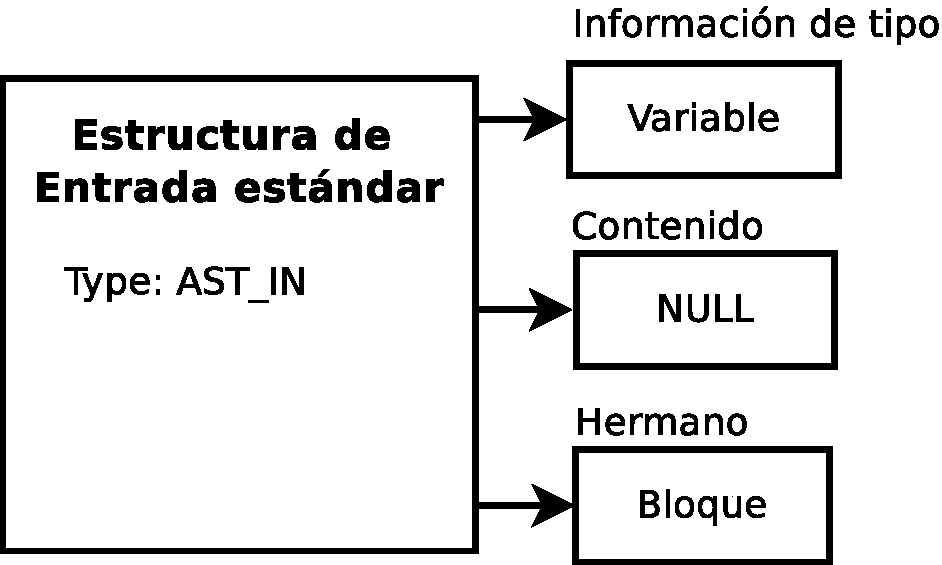
\includegraphics[width=0.33\textwidth]{images/ast_in.pdf}}
  \hspace{11mm}
  \subfloat[][Nodo de expresión de salida]{\label{fig:exprout}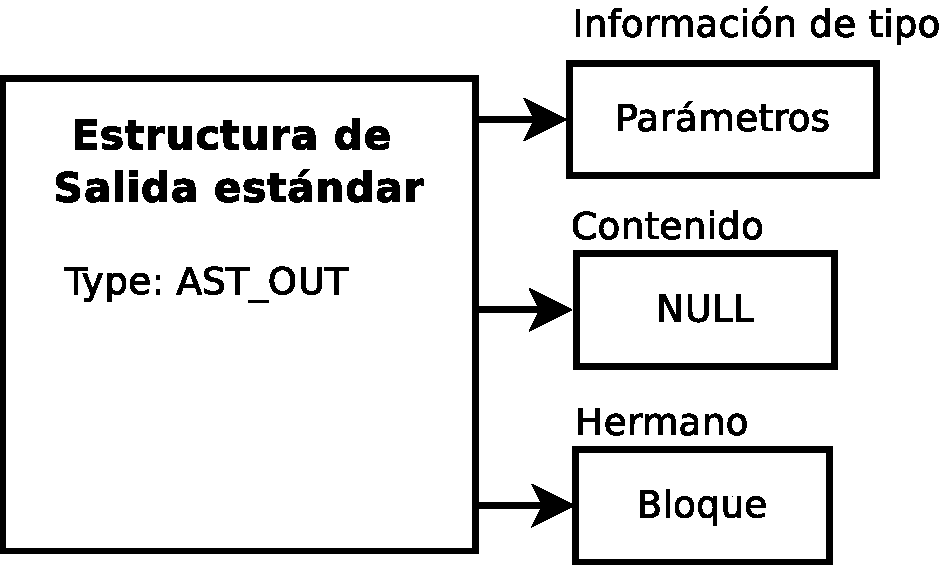
\includegraphics[width=0.33\textwidth]{images/ast_out.pdf}}
  \caption{Expresiones de entrada/salida}
  \label{fig:exprio}
\end{figure}

Para finalizar, se muestra un ejemplo de código en el lenguaje \textit{JAM} y el correspondiente árbol abstracto que se generaría a través del uso de todos los nodos explicados anteriormente. Es un ejemplo muy simple, pero da una buena idea de cómo se construye el árbol y de lo potente que puede ser su uso en la etapa de generación de código:

\begin{lstlisting}[language=jam]
void funcion(int n)
	int a
	int b = 7
	a = (2+n)*(10/b)
	return
end
\end{lstlisting}
\begin{figure}[H]
  \centering
	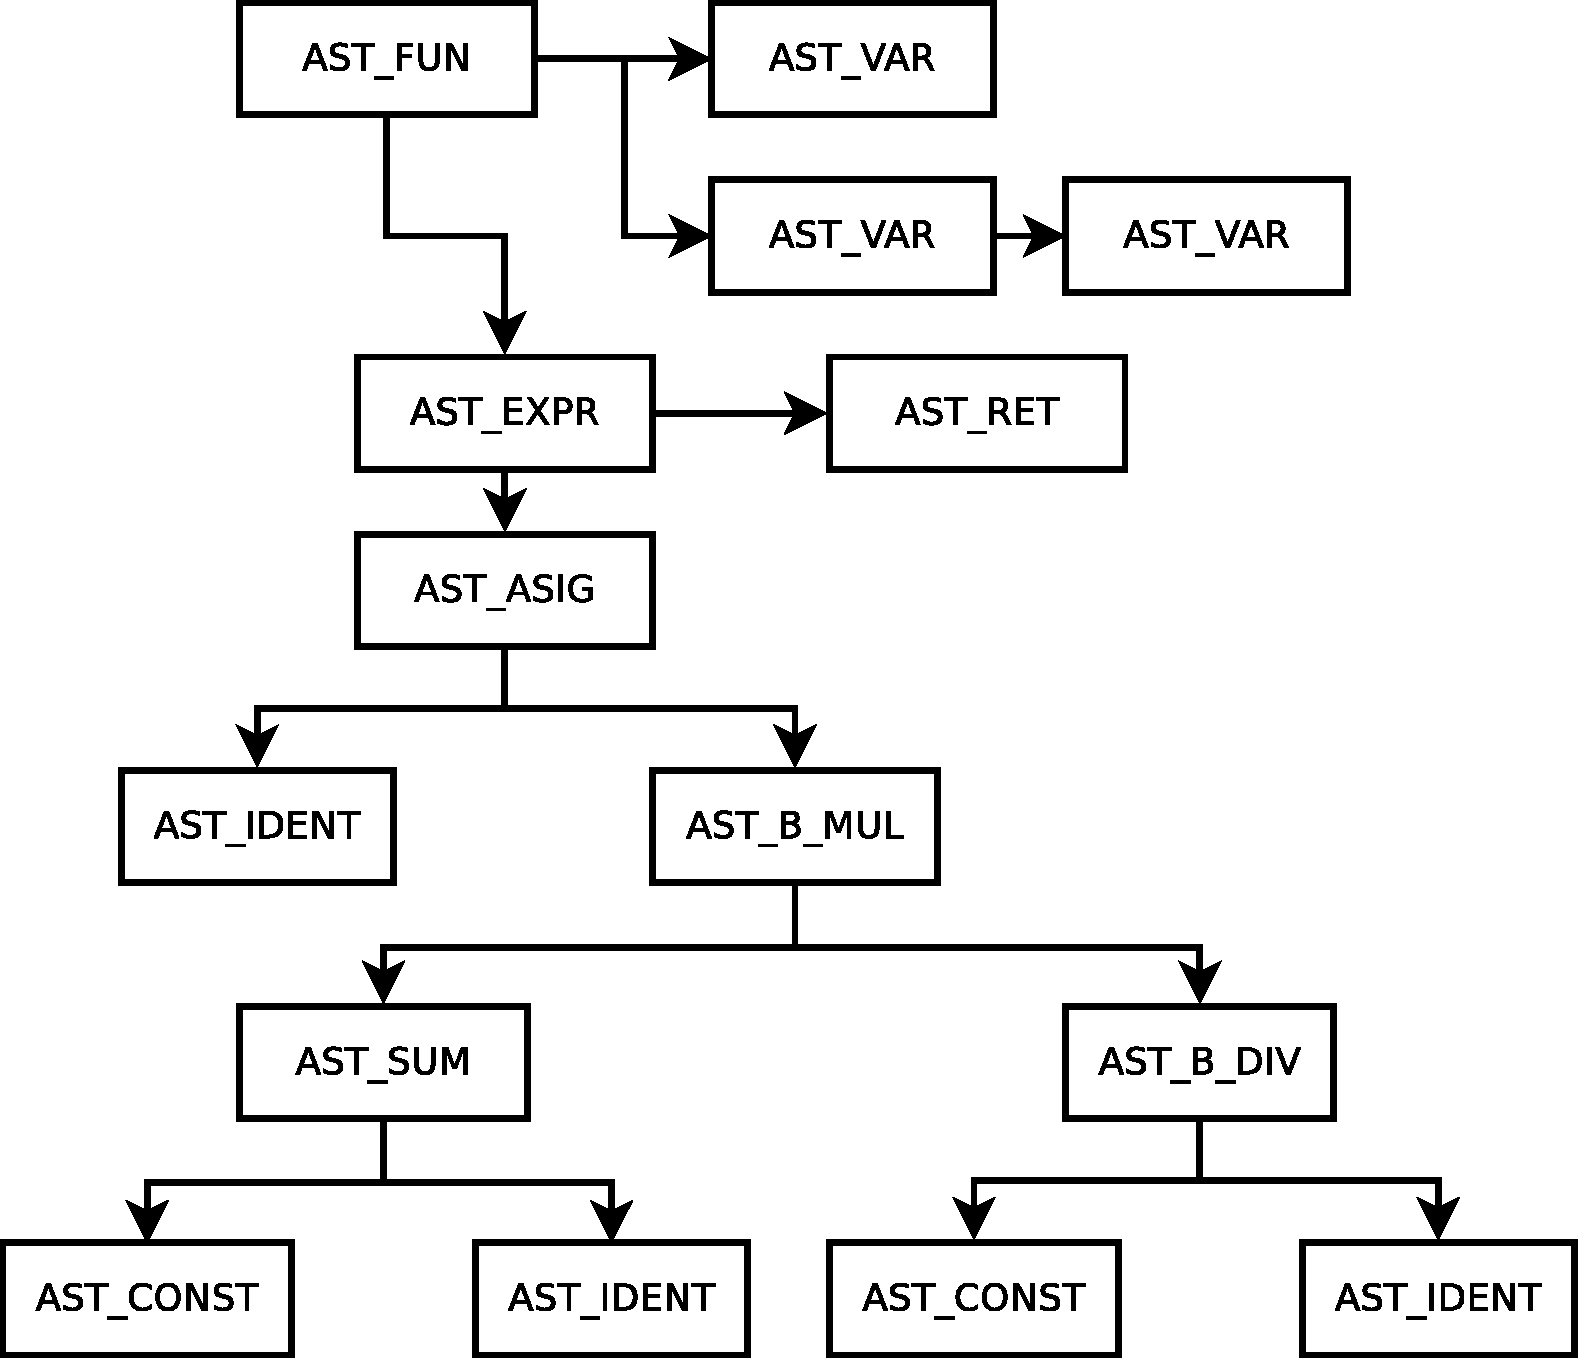
\includegraphics[width=0.5\textwidth]{images/ast.pdf}
  \caption{Ejemplo de árbol sintáctico abstracto formado}
  \label{fig:ast}
\end{figure}

\section{Generación de Código}

La generación de código es la etapa más compleja de todo el proceso de compilado. En nuestro caso traduciremos a código x86 con la sintaxis del ensamblador \textit{NASM}. Este ensamblador es multiplataforma y permite traducir de código ensamblador x86 a un fichero ejecutable en diversos formatos. Se ha conseguido que el código generado, al ser compilado, funcione correctamente y es algo de lo que nos sentimos extremadamente orgullosos.

El código \textit{x86} se divide en tres zonas principales. La primera de las zonas (.bss) es la zona de datos no inicializados. En esta zona se realiza una reserva de espacio en memoria y asignación de este espacio a un nombre. La segunda zona (.data) es la zona de datos inicializados en la que se asocia un nombre a un tipo de datos y a una constante de inicialización. Por último tendremos la zona de código (.text) que será aquella en la que todo el código funcional se sitúe.

El proceso, en consecuencia, se dividirá en 3 etapas principales, pero debido a que nosotros disponemos de una herramienta tan potente como el árbol sintáctico, nuestro proceso se dividirá en cuatro etapas. La primera será la generación de la zona de datos no inicializados. La segunda etapa será la generación de la zona de datos inicializados. La tercera etapa consistirá en una compresión del árbol sintáctico; en esta etapa se eliminarán las operaciones constantes, es decir, operaciones que se dan entre constantes y carece de sentido traducir a código máquina, además las variables de tipo ristra inicializadas y las ristras que se sitúen en el código se insertarán como nuevos nombres en la zona de datos inicializados y se sustituirán por el correspondiente identificador en donde toque. En esta tercera etapa también se generarán unas ristras para la salida por pantalla que se corresponderán con el formato de las ristras de la función \textit{printf} de la librería de \textit{C}. Estas ristras utilizarán la información de tipos de los parámetros de la operación de salida estándar.

\subsection{Zona de datos}
En la zona de datos del código x86 tendremos que situar todas y cada una de las variables globales del código, tanto inicializadas como no inicializadas. Además de ello, tendremos que crear nuevas variables para sustituir a variables locales que tengan ristras inicializadas o para sustituir a constantes ristra que se sitúan dentro del código. Debido a que el código de \textit{NASM} no permite que ciertos nombres sean utilizados, como por ejemplo los nombres de los registros de la máquina \textit{intel}, se ha optado por realizar una traducción de cada nombre a un nombre estándar \emph{var(n)} para variables y \emph{str(n)} para ristras. 

El acceso a las diferentes formas de variables será totalmente diferente para las variables globales que para las locales. Para las primeras con el nombre nos es suficiente ya que éste representa una dirección, sin embargo, para las variables locales la cosa se complica. Es por ello que se ha desarrollado un nuevo sistema de tablas de símbolos globales y locales en el que almacenar información parcial de las variables para el acceso en posteriores zonas del código.Además, este sistema de tablas de símbolos nos permite realizar la traducción entre los nombres definidos por el usuario y los nombres estándar utilizados por el compilador. La estructura de la tabla de símbolos es un \textit{hash}, como en el caso del analizador semántico, y el nodo de información tiene la siguiente estructura:

\begin{lstlisting}
struct var_info_ {
	char *name;
	local_type type;
	boolean vector;
	int offset;
	enum ast_subtype size;
};
\end{lstlisting}

El campo de nombre contendrá el nuevo nombre asociado al nombre antiguo de la variable, el tipo definirá si es una función, una variable o un parámetro. La variable vector nos permitirá distinguir si estamos accediendo a un vector y, en consecuencia, la forma en que debemos direccionarlo. El offset se utilizará para el acceso a variables locales y parámetros ya que éstos se encontrarán en la pila. El campo de tamaño contendrá el tipo de datos del nombre.

\subsubsection{Zona de datos no inicializados}
En la zona de datos no inicializados se encuentran todas las variables globales que no hayan sido inicializadas. Estas variables requieren que se les reserve una zona de memoria, de modo que puedan contener un dato del tamaño del tipo. La peculiaridad de definirlas en esta zona, como variables no inicializadas, es que automáticamente se inicializan a cero. A continuación se muestra un ejemplo de la traducción de cada una de las variables:
\begin{multicols}{2}
\begin{lstlisting}[language=jam,frame=single]
# No inicializadas: .bss
bool varboolni
char varcharni
int varintni
float varfloatni
int varintniv[5]
\end{lstlisting}

\begin{lstlisting}[frame=single]
section .bss
	var0	resb 1
	var1	resb 1
	var2	resd 1
	var3	resd 1
	var4	resd 5
\end{lstlisting}
\end{multicols}

Como se puede comprobar, el código máquina consiste en una terna nombre-tamaño-número. El procedimiento de creación de las variables requerirá que se les asigne un nuevo nombre y se genere su entrada en la tabla de símbolos global. El número de la terna corresponde con el número de elementos la variable, una variable normal tendrá un elemento y un vector el tamaño que se le haya asignado. Por último, el tamaño de cada elemento de la variable se determina mediante los modificadores \emph{resd} y \emph{resb} que se corresponden con tamaño 1 y 4 bytes respectivamente.

Para este trabajo, la función encargada deberá recorrer el campo de variables del nodo \textit{AST\_PROG}, en el que se definen las variables globales y seleccionar aquellas que no tengan información de tipo, ya que si estuvieran inicializadas contendrían una constante en dicha información de tipo. El proceso de generación de la zona de datos no inicializados corre a cargo de la función:
\begin{lstlisting}
void generate_bss(ast_node *tree);
\end{lstlisting}

\subsubsection{Zona de datos inicializados}

La zona de datos inicializados contendrá las diferentes variables globales inicializadas, variables locales inicializadas como ristras, y ristras como constantes en el código. De nuevo, se habrá de definir el tipo de dato de la variable que estamos inicializando. Al igual que antes disponemos de tipo para un byte (db) y tipo para cuatro bytes (dd). No será necesario definir el número de elementos que contendrá la variable ya que se determinará en función del número de constantes de inicialización separadas por coma:
\begin{multicols}{2}
\begin{lstlisting}[language=jam,frame=single]
# Inicializadas: .data
bool varbooli = true
char varchari = 'a'
int varinti = 20
float varfloati = 2.0
int varintiv[5] = [1, 2, 3, 4, 5]
char varstringi[12] = "Hello World\n"
\end{lstlisting}

\begin{lstlisting}[frame=single]
section .data
	var5	db 1
	var6	db 97
	var7	dd 20
	var8	dd 2.000000
	var9	dd 1, 2, 3, 4, 5
	var10	db "Hello World",10,"",0
\end{lstlisting}
\end{multicols}
En el ejemplo anterior se muestra que la ristra ha sido extrañamente descompuesta. Esto se debe a que, cuando creamos una ristra, debemos sustituir las secuencias de escape por su valor numérico y añadir el carácter nulo al final de la ristra. La extraña formación es un efecto colateral de la función que se encarga de esta tarea, pero son perfectamente válidas, por eso no se ha modificado tal comportamiento.

Cuando la función encargada de generar las variables de la sección de datos, debe realizar una llamada a la correspondiente función de compresión del árbol ya que existirán variables locales que hayan sido inicializadas como ristras y constantes ristra dentro del código. Ambas sufren una modificación: se les genera un nuevo nombre y una instancia en la zona de datos, pero eso se verá en la correspondiente sección. La función encargada de generar la zona de datos es la siguiente:

\begin{lstlisting}
void generate_data(ast_node *tree);
\end{lstlisting}

\subsection{Compresión del árbol}

La compresión del árbol es una tarea que puede dar para mucho si se pretende optimizar el código, pero en nuestro caso realizaremos unas pocas tareas simples. Inicialmente se recorrerá todo el árbol en busca de variables locales que hayan sido inicializadas con ristras. Para estas variables se creará una nueva variable global en la zona de datos inicializada con la ristra y su correspondiente entrada en la tabla de símbolos global. Posteriormente se buscarán constantes ristra y se les asignará un nombre en la zona de datos inicializada a la ristra y se creará una entrada en la tabla de símbolos. Las constantes ristra tendrán un nombre del tipo \emph{str(n)} y cuando se haya finalizado la generación de la información necesaria, se sustituirá el nodo de la constante por un nodo de identificador.
\begin{multicols}{2}
\begin{lstlisting}[language=jam,frame=single]
int main()
	char s[5] = "Hola\n"
	funcion("Adios\n")
	<++varchari++varfloati++varinti++"\n"
end
\end{lstlisting}

\begin{lstlisting}[frame=single]
section .data
	var11	db "Hola",10,"",0
	str0	db "Adios",10,"",0
	str1	db "",10,"",0
	str2	db "%c%f%d%s",0
\end{lstlisting}
\end{multicols}


Además de ello, y debido a que nuestro lenguaje proporciona una salida medianamente compleja, se creará una ristra del tipo de las esperadas por la función \textit{printf} para cada operación de salida existente. Esta ristra se creará con los tipos de los parámetros de impresión. Se añadirá un nuevo nombre en la tabla de símbolos y se añadirá un nodo de identificador en el puntero de contenido del operador de salida.

\begin{multicols}{2}
\begin{lstlisting}[language=jam,frame=single]
int main()
	varintni = 2*2*2*varinti
end
\end{lstlisting}

\begin{lstlisting}[language=jam,frame=single]
int main()
	varintni = (((2*2)*2)*varinti)
end
\end{lstlisting}
\end{multicols}

La siguiente tarea que realizará la función de compresión será eliminar, en la medida de lo posible, las operaciones entre constantes. Esto será posible cuando se encuentre un nodo de operador en el que ambos parámetros son constantes. Si el operador se asocia por la izquierda, y las constantes se sitúan a la derecha en la expresión, no se podrá realizar esta tarea ya que no se formarán nodos con operandos constantes, este comportamiento puede verse en el ejemplo inmediatamente inferior. En el ejemplo superior, podemos ver como la asociación por la izquierda se puede comprimir cuando las constantes están a la izquierda.


\begin{multicols}{2}
\begin{lstlisting}[language=jam,frame=single]
int main()
	varintni = varinti*2*2*2
end
\end{lstlisting}

\begin{lstlisting}[language=jam,frame=single]
int main()
	varintni = (((varinti*2)*2)*2)
end
\end{lstlisting}
\end{multicols}

Aunque esta función puede dar mucho más de si, nosotros no hemos implementado ninguna tarea más. Posibles optimizaciones pueden incluir la compresión de las operaciones constantes del caso anterior, siempre que fuera posible. La función encargada de comprimir el árbol es la siguiente:
\begin{lstlisting}
void tree_data_compress(ast_node *tree);
\end{lstlisting}

\subsection{Zona de código}
La zona de código es el apartado más importante de la generación de código. En esta zona se encontrará todo el grueso del programa y toda la complejidad de la aplicación. El procedimiento de traducción comenzará a recorrer cada una de las funciones, generando una tabla de símbolos para cada función. En dicha tabla de símbolos insertará la información relacionada con los parámetros y las variables. Posteriormente generará el código del bloque de la función.

\subsubsection{Traducción de funciones}

Antes de poder explicar la traducción de funciones se ha de explicar el funcionamiento de la pila en \textit{x86}. La pila, como toda pila, crece según se van añadiendo elemento. La peculiaridad de esta pila es que crece hacia direcciones de memoria inferiores. En consecuencia, cada vez que añadimos un elemento a la pila, el anterior estará en la dirección del tope de la pila sumado a un offset positivo.

En la pila de \textit{x86} existen dos punteros, el primero de ellos consiste en el \textit{ebp} que apunta a la dirección de \textit{ebp} anterior a la actual, seguido de la dirección de retorno de la función que ha realizado la llamada y de los parámetros de la función. Posteriormente tenemos el puntero \textit{esp} que señala al tope de la pila. 

En consecuencia, podemos utilizar la pila para almacenar las variables locales y parámetros de una función. Para el primer caso, se almacenarán justo después del puntero \textit{esp} y para el segundo caso, 8 bytes por encima del puntero \textit{ebp}:

\begin{lstlisting}
:    : 
|  5 | [ebp + 12] [esp + 24] (Segundo argumento)
| 10 | [ebp + 8]  [esp + 20] (Primer argumento)
| RA | [ebp + 4]  [esp + 16] (Direccion de retorno)
| FP | [ebp]      [esp + 8]  (Valor de EBP anterior)
|    | [ebp - 4]  [esp + 4]  (Segunda variable local)
|    | [ebp - 8]  [esp]      (Primera variable local)
:    :
\end{lstlisting}

Al uso de la pila para almacenar las variables locales de una función se le llama \emph{stack frame}. Esto se debe a que cada función adquiere un marco de memoria en función del número de parámetros y variables de que disponga. En consecuencia, para mantener la coherencia entre los \emph{stack frames} de cada función, es necesario reservar y devolver el espacio utilizado en la pila cada vez que se entra y sale de una función. Para esto tenemos las funciones \textit{enter}, \textit{leave} y \textit{ret}. La función \textit{enter} toma dos parámetros, el primero de ellos consiste en el tamaño en bytes que ocuparán las variables de la función. El segundo consistirá en el anidamiento de dicha función. La función \textit{leave} deshará lo realizado por \textit{enter}. Finalmente, la función \textit{ret}, retornará de la función tomando un parámetro que consistirá en el número de bytes que ocupan los parámetros de dicha función:

\begin{lstlisting}
	enter 0,0
	leave
	ret 4
\end{lstlisting}
En general, las funciones enter y leave son macros que internamente realizan las operaciones necesarias. Enter inserta el puntero \textit{ebp} en la pila, lo sustituye por la actual posición del puntero \textit{ebp} anterior y reserva la memoria especificada por el primer parámetro de la función enter. La función leave, recupera el puntero \textit{ebp} y recupera el tope anterior de la pila:
\begin{lstlisting}
push ebp
mov ebp, esp
sub esp, 0

mov esp, ebp
pop ebp
ret 4 
\end{lstlisting}

En consecuencia, al inicio y final de cada función, así como en los lugares en los que exista un salto de retorno, tendremos que añadir los códigos enter, leave y ret adecuados a la función. Todo lo anteriormente explicado funciona como un estándar, es decir, se espera que los programadores en ensamblador apliquen en sus programas este comportamiento. Por un lado tenemos los \emph{stack frames} que consisten en los marcos de variables locales y por otros las \emph{calling conventions} que son unas reglas que especifican como se le pasarán los parámetros a una función y como se retornará el valor de la misma.

Una vez explicado esto estamos en disposición de entender el procedimiento de traducción de funciones. El primer paso para la creación de la función consistirá en la creación de la tabla de símbolos local. Posteriormente se insertará el nombre de la función en la tabla de símbolos global por lo cual se le asignará un nuevo nombre, a menos que se trate de la función \textit{main}. 

Una vez hecho esto, se debe obtener el tamaño y offset para cada variable y parámetro de la función. Los parámetros y las variables están claramente separados en la información de tipo del nodo de función, pero el procedimiento es el mismo. En primer lugar existirán dos variables que se corresponderán con el puntero \textit{ebp} y el puntero \textit{esp}. Todos los parámetros serán accedidos mediante un offset sobre el \textit{ebp}+8 y todas las variables mediante un offset sobre \textit{esp}.

\begin{enumerate}
\item Se obtiene el siguiente parámetro o variable.
\item Se crea un nuevo símbolo en la tabla de símbolos local en el que se contenga la información de la variable o parámetro (incluyendo si es una variable o un parámetro) y sobre todo la información del offset, que se corresponderá con el contenido de la variable \textit{esp} o \textit{ebp}, según fuera variable o parámetro.
\item Se calculará el tamaño de la variable en función del tipo de datos y el número de elementos que contiene (en caso de que fuera vectorial). En caso de ser una variable cuyo tipo de datos requiera 1 byte, éste se alineará a múltiplo de 4 (p.e. char v[9] ocupará 12 bytes). Este tamaño se sumará a la variable \textit{esp} o \textit{ebp} según corresponda.
\item Se almacenará en una pila una o múltiples ristras que se corresponderán con el código ensamblador necesario para inicializar la variable en caso de que tuviera inicialización.
\item Se retorna a 1 hasta que no haya más parámetros/variables.
\end{enumerate}

Para la generación de la función será necesario utilizar toda la información que se ha ido obteniendo para generar una estructura con la siguiente forma:

\begin{lstlisting}
[Nombre funcion]:
	enter [esp], 0
	[Inicializaciones]
	
	leave
	ret [ebp-8]
\end{lstlisting}

Donde el nombre de la función será aquel que haya sido asignado en la creación del nombre global, la variable \textit{esp} de la función \textit{enter} será aquella que hemos utilizado para obtener el \textit{offset} de cada variable. Las inicializaciones será las que se hayan ido insertando en la pila y el \textit{ebp-8} será la misma variable que se utilizó para calcular el offset de los parámetros.
\begin{multicols}{2}
\begin{lstlisting}[language=jam,frame=single]
void funcion(char s[])
	int i
	
	[Contenido]
end
\end{lstlisting}
\begin{lstlisting}[frame=single]
fun0:
	enter 4,0
	[Contenido]
	leave
	ret 4
\end{lstlisting}
\end{multicols}

Naturalmente, ésta es la estructura de la función, pero falta un elemento fundamental que es el contenido de la función que irá situado entre las inicializaciones y el \textit{leave}. Para la generación de este apartado se realizará una llamada a la siguiente función:

\begin{lstlisting}
void gen_text_content(ast_node *tree,int  offset);
\end{lstlisting}

La función de generación de contenido será la principal encargada de generar código para todos los bloques existentes. Esta función discriminará entre expresiones, bucles, saltos o sentencias de selección, llamando a las funciones que generarán el código correspondiente. Más adelante se verá que todas las estructuras que contienen bloques hacen uso de esta misma función.

Finalmente, especificar que la función encargada de la generación del código correspondiente a las funciones en \textit{JAM} es la primera en una jerarquía de funciones que se encargan de generar todo el código. Su prototipo es el siguiente:

\begin{lstlisting}
void generate_text(ast_node *tree);
\end{lstlisting}

\subsubsection{Traducción de bucles y saltos}
La generación de bucles requerirá mantener una serie de contadores con el objetivo de generar las etiquetas adecuadas para cada bucle. Se permiten múltiples niveles de bucles y múltiples bucles en una misma función, en consecuencia, mantendremos un contador del número de bucles que existen y un contador del bucle en el que nos encontramos que valdrá \textit{-1} cuando no nos encontremos en ningún bucle:
\begin{lstlisting}
int loop_id = 0;
int loop_level = -1;
\end{lstlisting}

En las funciones de generación de bucles se utilizará el \textit{id} de bucle para generar las etiquetas relacionadas con el bucle actual y el \textit{loop level} para que instrucciones contenidas dentro del bloque del bucle puedan conocer el bucle en el que se encuentran. La idea principal consistirá en que las funciones de bucles mantendrán su \textit{id} para la generación de etiquetas y guardarán el \textit{loop level} anterior y lo sustituirán por su id de bucle; una vez fuera del bucle se devolverá el \textit{loop level} anterior. De este modo se mantendrá la coherencia con las etiquetas dentro de los bucles anidados.

Las etiquetas de bucle tienen una cierta coherencia, para empezar, la etiqueta \emph{ls(n)} indica el principio de la siguiente iteración, la etiqueta\emph{lr(n)} indica el final del bucle y la etiqueta \emph{l(n)} del bucle for simplemente sirve para evaluar la condición del bucle tras un paso. A continuación se muestra el código generado para un bucle \textit{while} en el que el resultado de su condición se almacenará en el registro \textit{eax} y se hará una comprobación para continuar o salir del bucle:

\begin{multicols}{2}
\begin{lstlisting}[language=jam,frame=single]
	while( [Condicion] )
		[...
		 ...
		 Contenido
		 ...
		 ...]
	end
\end{lstlisting}
\begin{lstlisting}[frame=single]
ls(n):
	[Condicion -> eax]
	cmp eax, 0
	jz lr(n)
	[Contenido]
	jmp ls(n)
lr(n):
\end{lstlisting}
\end{multicols}

En el bucle for, sin embargo, disponemos de tres expresiones de interés. La primera, la inicialización, se dará justo antes del bucle y no se repetirá de nuevo. La condición se realizará justo al principio del bucle, después de la etiqueta \emph{l(n)}. El paso se realizará al final del bucle, en la etiqueta \emph{ls(n)}. Esta etiqueta representa el principio del paso del bucle.
\begin{multicols}{2}
\begin{lstlisting}[language=jam,frame=single]
	for([Inicializacion] ; [Condicion] ; [Paso])
		[...
		 ...
		 ...
		 Contenido
		 ...
		 ...
		 ...
		 ...]
	end
\end{lstlisting}
\begin{lstlisting}[frame=single]
	[Inicializacion]
l(n):
	[Condicion -> eax]
	cmp eax, 0
	jz lr(n)
	[Contenido]
ls(n):
	[Paso]
	jmp l(n)
lr(n):
\end{lstlisting}
\end{multicols}

Cuando se ejecuta el contenido y el paso, el bucle salta directamente a la parte de arriba, en la que se evalúa la condición \emph{l(n)} \emph{ls(n)}. Cuando la condición del bucle no se cumple, se realiza un salto directamente al final del bucle, a \emph{lr(n)}.

Como consecuencia de las etiquetas de los bucles, las sentencias \textit{continue} y \textit{break} tendrán una traducción directa y la única información necesaria será el \textit{loop level}:

\begin{multicols}{2}
\begin{lstlisting}[language=jam,frame=single]
	continue
	break
\end{lstlisting}
\begin{lstlisting}[frame=single]
	jmp ls([loop_level]);
	jmp lr([loop_level]);
\end{lstlisting}
\end{multicols}

Finalmente, la traducción del retorno de función requerirá la variable \textit{ebp} explicada anteriormente para que se eliminen los parámetros de la función correctamente. Según las \emph{calling conventions} todas las funciones retornarán su valor en el registro \textit{eax}:

\begin{multicols}{2}
\begin{lstlisting}[language=jam,frame=single]

	return [Expresion]
	...
\end{lstlisting}
\begin{lstlisting}[frame=single]
	[Expresion -> eax]
	leave
	ret [ebp - 8]
\end{lstlisting}
\end{multicols}
La función que se encarga de la traducción de los saltos será la propia función de generación de contenido ya que esta traducción es extremadamente simple. La funciones que generarán los bucles serán las siguientes:

\begin{lstlisting}
void gen_text_for(ast_node *node, int offset);
void gen_text_while(ast_node *node, int offset);
\end{lstlisting} 
\subsubsection{Traducción de sentencias de control}

El proceso de traducción de las sentencias de control es similar para ambos tipos de sentencias. Empezando por el \textit{if}, mantendremos un contador para poder definir etiquetas mutuamente excluyentes. Además, como una sentencia \textit{if} puede venir precedida de múltiples \textit{elsif} o un \textit{else}, también se dispondrá de un contador interno para cada \textit{if}, mediante el cual se podrá ir saltado de condición en condición en busca de la que coincida, o del \textit{else}.

La traducción del \textit{if} más simple, dispone de una etiqueta de final de \textit{if}. La condición del \textit{if} será una expresión cuyo resultado se encontrará en el registro \textit{eax}, se evaluará este resultado y se procederá con el cuerpo de la sentencia \textit{if} o se saltará hacia la etiqueta de final de \textit{if}:

\begin{multicols}{2}
\begin{lstlisting}[language=jam,frame=single]
	if([Condicion])
		[...
		 Contenido
		 ...]
	end
\end{lstlisting}
\begin{lstlisting}[frame=single]
	[Condicion]
	cmp eax, 0
	jz endif(n)
	[Contenido]
endif(n):
\end{lstlisting}
\end{multicols}

La combinación de \textit{if} y \textit{else} es ligeramente más compleja. Para empezar, la condición del \textit{if} saltará directamente a la etiqueta \textit{if(n)(i)} que se corresponderá con la siguiente sentencia \textit{elsif/else}. En este caso, como el \textit{else} sucederá al cuerpo del \textit{if}, se añadirá una etiqueta para ir directamente al final del \textit{if}. En el \textit{else} no se evaluará ningún tipo de condición, sino que se procederá directamente a ejecutar su contenido:

\begin{multicols}{2}
\begin{lstlisting}[language=jam,frame=single]
	if([Condicion])
		[...
		 Contenido 1
		 ...]
	else
		[...
		 Contenido 2
		 ...]
	end
\end{lstlisting}
\begin{lstlisting}[frame=single]
	[Condicion]
	cmp eax, 0
	jz if00
	[Contenido 1]
	jmp endif0
	
if00:
	[Contenido 2]
endif0:
\end{lstlisting}
\end{multicols}

El caso de múltiples \textit{elsif} y \textit{else} es análogo al anterior, la única excepción es que en este caso se contienen múltiples etiquetas del tipo \textit{if(n)(i)} y se irá saltado de una a otra hasta que alguna sea verdadera o se llegue al \textit{else}. De nuevo, habrá múltiples etiquetas al final del cuerpo de cada \textit{if/elsif} que conducirán directamente al final del \textit{if}:
\begin{multicols}{2}
\begin{lstlisting}[language=jam,frame=single]
	if([Condicion 1])
		[...
		 Contenido 1
		 ...]
	elsif([Condicion 2])
		[...
		 Contenido 2
		 ...
		 ...]
	elsif([Condicion 3])
		[...
		 Contenido 3
		 ...
		 ...]
	else
		[...
		 Contenido 4
		 ...
		 ...]
	end
\end{lstlisting}
\begin{lstlisting}[frame=single]
	[Condicion 1]
	cmp eax, 0
	jz if00
	[Contenido 1]
	jmp endif0
if00:
	[Condicion 2]
	cmp eax, 0
	jz if01
	[Contenido 2]
	jmp endif0
if01:
	[Condicion 3]
	cmp eax, 0
	jz if02
	[Contenido 3]
	jmp endif0
if02:
	[Contenido 4]
endif0:
\end{lstlisting}
\end{multicols}
	
El desarrollo de la sentencia \textit{switch} es análoga al de la sentencia \textit{if}, excepto por pequeñas peculiaridades. Para empezar, la expresión del \textit{switch} se evaluará y se almacenará en el registro \textit{eax} que luego será utilizado para realizar comparaciones con las constantes de cada case hasta que alguna de ellas encaje, en caso de no ser así y de existir un \textit{default} se procederá por esta vía.

En el ejemplo a continuación se puede observar como las etiquetas del \textit{switch} son similares a las del if, con dos números, el primer consiste en el número de \textit{switch} y el segundo en el número de \textit{case}. En el ejemplo de abajo sólo existe una sentencia \textit{default}, por lo que se procede directamente a ejecutar el contenido de la misma:
\begin{multicols}{2}
\begin{lstlisting}[language=jam,frame=single]
	switch([Expresion])
	default:
		[Contenido]
	end
\end{lstlisting}
\begin{lstlisting}[frame=single]
	[Expresion]
case00:
	[Contenido]
endswtch0:
\end{lstlisting}
\end{multicols}

En el ejemplo siguiente se puede observar la traducción de una sentencia \textit{switch} con múltiples case. El código resultante realizará las comparaciones necesarias para decidir si se debe ejecutar o no el código contenido en el case o se procede con el siguiente \textit{case} o \textit{default}. De nuevo, al final de cada case existirá una etiqueta para salir de la sentencia \textit{switch}:

\begin{multicols}{2}
\begin{lstlisting}[language=jam,frame=single]
	switch([Expresion])
	case [Constante 1]:
		[...
		 Contenido 1
		 ...]
	case [Constante 2]:
		[...
		 Contenido 2
		 ...]
	default:
		[...
		 Contenido 3
		 ...]
	end
\end{lstlisting}
\begin{lstlisting}[frame=single]
	[Expresion]
case00:
	cmp eax, [Constante 1]
	jne case01
	[Contenido 1]
	jmp endswtch0
case01:
	cmp eax, [Constante 2]
	jne case02
	[Contenido 2]
	jmp endswtch0
case02:
	[Contenido 3]
endswtch0:
\end{lstlisting}
\end{multicols}

Las funciones que se encargarán de esta tarea son las que se ven a continuación. Es necesario recalcar que todas estas funciones serán llamadas por la función de generación de contenido:
\begin{lstlisting}
void gen_text_switch(ast_node *tree, int offset);
void gen_text_if(ast_node *tree, int offset);
\end{lstlisting}
\subsubsection{Traducción de expresiones}

La traducción de expresiones será un proceso bastante más complejo que la traducción del resto del código. Para empezar, en esta etapa aparecen problemas como la carencia de registros. Para este problema particular se ha desarrollado una serie de funciones que nos permitirán realizar almacenamiento temporales en memoria y, de este modo, tener registros libres siempre que sea necesario.

La solución para este problema es el denominado derramamiento de registros, que consiste en almacenar el contenido de un registro en memoria cuando no quedan registros libres que se puedan utilizar. En este caso, como en \textit{x86} sólo disponemos de 8 registros, de los cuales sólo podemos estar seguros de que no vamos a causar un destrozo usando 4 de ellos. En consecuencia, el sistema de derramamiento de registros que se ha desarrollado consiste en un vector de tamaño 4 y en un tipo de datos con el cual distinguir el registro que vamos a utilizar de forma intuitiva y poco costosa:

\begin{lstlisting}
enum reg_name_ {NAR=-1, EAX=0, EBX=1, ECX=2, EDX=3};
typedef enum reg_name_ reg_name;

int reg_buffer[4] = {0, 0, 0, 0};
\end{lstlisting}

Mediante el vector de registros podremos reservar registros u obtener su estado en un momento dado. Para reservar registros existen dos maneras principales. La primera es saber de antemano qué registro se necesita, en este caso podemos hacer una llamada a la función \textit{reg\_alloc} con el nombre del registro que queremos reservar. Por otro lado, podemos querer reservar un registro aleatorio, para ese caso tenemos la función reg\_ralloc. La primera de ellas simplemente reserva el registro sin tener en cuenta si ya está siendo usado, la segunda devolverá el nombre \textit{NAR} (Not a register) como aviso de que no existen registros libres.
\begin{lstlisting}
reg_name reg_alloc(reg_name reg);
reg_name reg_ralloc();
\end{lstlisting}

Para ambos casos hay solución. Para el primer caso tenemos la función \textit{reg\_state} que nos devolverá el estado del registro por el que consultemos. Para el caso en que \textit{reg\_alloc} nos informe de que no quedan registros libres, lo que haremos será coger el siguiente registro del que se nos ha solicitado utilizar para el retorno del dato mediante la función \textit{reg\_next}.
\begin{lstlisting}
int reg_state(reg_name reg);
reg_name reg_next(reg_name reg);
\end{lstlisting}

Siempre que llegamos a una situación de este tipo, lo que se debe hacer es utilizar el registro que necesitamos o que se nos ha proporcionado (que estará ocupado) e insertarlo en la pila. En este caso, el campo offset de todas y cada una de las variables perderá coherencia, es por eso que las funciones de generación de código \textit{JAM} disponen de un parámetro offset que permitirá mantener esta coherencia perdida. Una vez se haya insertado el dato del registro en la pila, somos libres de utilizar ese registro como así lo queramos siempre y cuando al finalizar el uso retornemos el valor a su sitio.

En caso de que existan registros libres y lo hayamos reservado, podremos liberarlo mediante la función \textit{reg\_free}. De este modo se mantiene la coherencia en la pila de registros y, con 4 registros y la pila, seremos capaces de resolver cualquier expresión aritmética que se nos presente.
\begin{lstlisting}
reg_name reg_free(reg_name reg);
\end{lstlisting}

Explicar la traducción de todas y cada una de las expresiones puede llegar a ser una tarea hercúlea, es por ello que se explicará por encima como se realiza el proceso de traducción de forma general. Para empezar, la raíz de una expresión será siempre un operador, este operador puede ser unario o binario, en el caso de ser binario tendrá dos operandos que podrán ser a su vez operadores, variables o llamadas a funciones. El proceso de traducción comenzará con la raíz y un registro (generalmente \textit{eax}), se realizará una llamada a evaluar la expresión del primer operando y almacenarla en el registro que se nos ha proporcionado y en el que se espera que se almacene el valor. 

Posteriormente, se obtendrá un registro, mediante lo explicado anteriormente, para el siguiente operando, en caso de no haber se realizará el derramamiento correspondiente y se incrementará el offset en 4 ya que nuestra pila está alineada. El procedimiento habrá seguido su curso y ya se habrá creado el código para obtener los resultados esperados en los registros especificados. En este momento tocará crear el código para la operación actual con los dos registros de que disponemos.

En algunos casos, como en los desplazamientos o la división, se requiere del uso de unos registros en particular. El procedimiento, en general, es análogo, pero en vez de solicitar un registro aleatorio y derramar un registro cualquiera, se realizará sobre estos registros que necesitemos. Finalmente, las expresiones han de situar el resultado final en el registro que se haya especificado.

\begin{multicols}{2}
\begin{lstlisting}[language=jam,frame=single]
	varintni = 2 * varinti + varchari
	...
	...
	...
	...
	...
	...
\end{lstlisting}
\begin{lstlisting}[frame=single]
	mov eax, 2
	mov ebx, dword [var7]
	imul eax, ebx
	movsx ebx, byte [var6]
	add eax, ebx
	mov dword [var2], eax
	mov eax, dword [var2]
\end{lstlisting}
\end{multicols}
En este ejemplo se puede ver el procedimiento que ha seguido el compilador para realizar esa simple operación. Puede parecer excesivamente complejo y se podría realizar en muchas menos líneas, pero el compilador es capaz de utilizar múltiples registros, derramándolos si fuera necesario, para realizar operaciones aritméticas tan largas como se nos presenten. La función encargada de esta gran tarea es la siguiente:

\begin{lstlisting}
void gen_text_expr(ast_node *tree, reg_name reg, int offset);
\end{lstlisting}
\subsubsection{Traducción de expresiones de entrada salida}

Las expresiones de entrada y de salida no consistirán más que en una llamada a una función. La expresión de entrada sólo permite una entrada de un carácter. Si en algún momento se quiere realizar una entrada más sofisticada en el lenguaje \textit{JAM} se puede hacer una función que lea carácter a carácter y realiza con esa información lo que se necesite. Esta función hará una simple llamada a la función de la librería de \textit{C} \textit{getchar}. Esta función no requiere parámetros de entrada y retornará la información necesaria en el registro \textit{eax}:
\begin{multicols}{2}
\begin{lstlisting}[language=jam,frame=single]
>++varcharni
...
\end{lstlisting}
\begin{lstlisting}[frame=single]
	call getchar
	mov byte [var1], al
\end{lstlisting}
\end{multicols}

Para la impresión por pantalla se utiliza la función \textit{printf}, como se explicó anteriormente, esta función requiere de una ristra ha sido previamente creada por la función de compresión del árbol. El procedimiento sigue las \emph{calling conventions}, insertará los parámetro de la función en la pila y en el tope insertará el puntero a la ristra de \textit{printf}:
\begin{multicols}{2}
\begin{lstlisting}[language=jam,frame=single]
<++"Hola\n"
...
...
...
...
...
...
\end{lstlisting}
\begin{lstlisting}[frame=single]
	sub esp, 8
	mov eax, dword str11
	mov dword [esp + 4], eax
	mov eax, dword str12
	mov dword [esp], eax
	call printf
	add esp, 8
\end{lstlisting}
\end{multicols}

\noindent La función encargada de realizar esta tarea será la siguiente:

\begin{lstlisting}
void gen_text_io(ast_node *tree);
\end{lstlisting}
\subsubsection{Llamadas a funciones}

Las llamadas a funciones procederán acorde con las \emph{calling conventions}. En primer lugar, como los parámetro de una llamada a función pueden ser expresiones, se irán evaluando una a una dichas expresiones y el resultado será insertado en la pila en el orden correspondiente. Cuando todos los parámetro se hayan insertado correctamente en la pila, se procederá a realizar una llamada a la función:
\begin{multicols}{2}
\begin{lstlisting}[language=jam,frame=single]
funcion("0123456789", 2)
...
...
...
...
\end{lstlisting}
\begin{lstlisting}[frame=single]
	mov eax, 2
	push eax
	mov eax, dword str8
	push eax
	call fun0
\end{lstlisting}
\end{multicols}

Siguiendo las \emph{calling conventions} todos los resultados de funciones se retornarán en el registro \textit{eax}, es por ello que si este registro está siendo usado antes de una llamada a función se debe realizar el correspondiente derramamiento.

\subsubsection{Lectura y escritura de variables}

Para finalizar la traducción de código, se hablará de la lectura y escritura de variables. La escritura de variables consistirá en un proceso de almacenamiento de un registro en una zona de memoria. Esta zona de memoria especificada puede resultar ser una variable global, una variable local, o un parámetro. En general, la sintaxis de la expresión de un almacenamiento es la siguiente:

\begin{lstlisting}
mov [Nombre + Registro_1 + Offset], Registro_2
\end{lstlisting}
\noindent Dónde:
\begin{itemize}
\item \textbf{Nombre:} puede ser el nombre de una variable global, el registro \textit{esp} en caso de ser una variable local o el registro \textit{ebp} en caso de ser un parámetro de una función.
\item \textbf{Registro\_1:} se utilizará únicamente si la variable sobre la que se va a escribir es un vector y está siendo direccionada mediante una expresión. Este registró contendrá el valor del índice del vector.
\item \textbf{Offset:} en caso de ser una variable o un parámetro, este offset se utilizará para determinar el lugar respecto a los registros \textit{ebp} o \textit{esp}, en el que se encuentra la variable o parámetro que queremos utilizar.
\item \textbf{Registro\_2:} contendrá el valor que se quiere almacenar en memoria.
\end{itemize}


Un ejemplo de esto pueden ser los siguientes:
\begin{multicols}{2}
\begin{lstlisting}[language=jam,frame=single]
varintni = 2
...
...
varlocal=2
...
...
varintniv[5] = 2
...
...
...
\end{lstlisting}
\begin{lstlisting}[frame=single]
	mov eax, 2
	mov dword [var2], eax

	mov eax, 2
	mov dword [esp + 0], eax
	
	mov eax, 2
	mov ebx, 5
	sal ebx, 2
	mov dword [var4 + ebx], eax
\end{lstlisting}
\end{multicols}

Se puede observar que se realiza un desplazamiento, esto se debe a que el índice se debe multiplicar por cuatro para acceder a la posición de memoria correspondiente a un vector de enteros. La función encargada de realizar esta tarea es la siguiente:

\begin{lstlisting}
void gen_text_var_write(ast_node *ident, reg_name reg, int offset);
\end{lstlisting}

De forma análoga a la escritura tenemos la lectura. El formato de una lectura será el siguiente:
\begin{lstlisting}
mov Registro_1, [Nombre + Registro_2 + Offset]
\end{lstlisting}
\noindent Dónde:
\begin{itemize}
\item \textbf{Nombre:} puede ser el nombre de una variable global, el registro \textit{esp} en caso de ser una variable local o el registro \textit{ebp} en caso de ser un parámetro de una función.
\item \textbf{Registro\_1:} será el registro en el que se almacene el valor de la variable que se desea leer.
\item \textbf{Offset:} en caso de ser una variable o un parámetro, este offset se utilizará para determinar el lugar respecto a los registros \textit{ebp} o \textit{esp}, en el que se encuentra la variable o parámetro que queremos utilizar.
\item \textbf{Registro\_2:} se utilizará únicamente si la variable sobre la que se va a escribir es un vector y está siendo direccionada mediante una expresión. Este registró contendrá el valor del índice del vector.
\end{itemize}


Ejemplos de lectura de variables pueden ser los siguientes:

\begin{multicols}{2}
\begin{lstlisting}[language=jam,frame=single]
varintni
...
varlocal
...
varintniv[5]
...
...
\end{lstlisting}
\begin{lstlisting}[frame=single]
	mov eax, dword [var2]
	
	mov eax, dword [esp + 0]
	
	mov eax, 5
	sal eax, 2
	mov eax, dword [var4 + eax]
\end{lstlisting}
\end{multicols}

\noindent La función encargada de realizar esta tarea será la siguiente:

\begin{lstlisting}
void gen_text_var_read(ast_node *ident, reg_name reg, int offset);
\end{lstlisting}

Se puede observar como a las funciones de acceso a variables se les ha incluido el offset. Estas funciones dependen de forma directa a este offset ya que se derrama algún registro en las funciones anteriores, es necesario mantener esta información para que los accesos a la pila sean coherentes.

\subsection{Pruebas}

Para comprobar que los resultados fueron los correctos se realizaron una serie de pruebas, muchas de ellas pruebas puntuales, pero las pruebas definitivas fueron los ficheros que se encuentran en el anexo. La batería de pruebas principal fue determinante para depurar el compilador y comprobar que el código se generaba correctamente.

Por otro lado, otro de los motivos por los que se sabe que todo el código funciona de forma correcta y que el compilador está realizando una generación coherente es debido a que todo el código generado es ensamblable mediante el ensamblador \textit{NASM}. El linkado se realizará posteriormente con el propio \textit{gcc}.

Entre las pruebas hay dos que son bastante importantes. El primero de ellos es la miniaplicación que se desarrollo junto con la especificación, aunque ligeramente cambiada debido a errores que se han ido corrigiendo. Consiste en el problema del viajante resuelto mediante la generación de todas las combinaciones posibles y la comprobación de la distancia. La prueba del \textit{tsp} genera un código máquina bastante generoso, de aproximadamente 600 líneas, con lo cual pegarlo aquí carecería de sentido, pero se incluye junto con el resto de los ficheros de prueba el código máquina de la compilación de cada prueba.

La segunda prueba de importancia es la del ordenamiento de burbuja. Es otra de las pruebas que verificaron que el compilador de \textit{JAM} genera un código correcto y coherente. No genera tanto código como el problema del viajante, pero no deja de ser lo suficientemente grande como para que pegar el código en esta memoria carezca de sentido.

En la sección de funcionamiento del compilador se explicarán brevemente cada una de las opciones del compilador, así como los requisitos para generar un ejecutable.
\section{Funcionamiento de \textit{jamcc}}
En esta sección se explicará el funcionamiento del compilador del lenguaje \textit{JAM}. El compilador es simple de usar, tan sólo acepta unas pocas opciones, pero es conveniente explicarlas para evitar confusión:
\begin{itemize}
\item \emph{-i, --input}: imprime un mensaje con información de ayuda en el uso del compilador.
\item \emph{-o, --output}: esta opción permite selección el nombre del fichero de salida.
\item \emph{-a, --assemble}: esta opción permite generar un ejecutable a partir del código saliente del compilador de \textit{JAM}. Requiere \textit{NASM} para el ensamblado y \textit{gcc} para el linkado.
\item \emph{-v, --version}: imprime un mensaje con información sobre la licencia del compilador, la versión ya se habrá imprimido al ejecutar el compilador.

\begin{lstlisting}
Copyright (C) 2010 Anil Motilal Mahtani Mirchandani(anil.mmm@gmail.com)
                   Mikel Ganuza Estremera(migaes.mail@gmail.com)
License GPLv3+: GNU GPL version 3 or later <http://gnu.org/licenses/gpl.html>
This is free software: you are free to change and redistribute it.
There is NO WARRANTY, to the extent permitted by law.
\end{lstlisting}
\item \emph{-h, --help}: imprime un mensaje con información de ayuda en el uso del compilador.
\begin{lstlisting}
Usage: jamcc [-vhioa]

	-v, --version			Prints version information
	-h, --help				Prints this help
	-i, --input FILE	Input file name
	-o, --output FILE	Output file name
	-a, --assemble		Creates linux executable file

Report bugs to anil.mmm@gmail.com.
\end{lstlisting}
\end{itemize}

\section{Conclusión}
La construcción de un compilador ha sido una tarea hercúlea.En un principio estábamos dispuestos a seguir los consejos para la correcta y simple construcción del compilador ofrecidos por el profesor, pero a medida que se iba desarrollando cada etapa, nos íbamos dando cuenta de que era necesario ir un paso más allá para poder realizar un trabajo que nos llenara y nos hiciera aprender. Finalmente, podemos asegurar que si algo hemos ganado realizando el compilador ha sido un gran conocimiento en el desarrollo de compiladores mediante el uso de las herramientas existentes, así como en el uso de estructuras tan elegantes como el árbol sintáctico abstracto.

Decidimos no utilizar el código Q, no porque no sea un código válido, sino porque ya habíamos trabajado con él en una asignatura anterior mediante la completa implementación de un intérprete de este mismo lenguaje. Es por ello que decidimos probar algo diferente y quizás más a bajo nivel.

Además de ello, la decisión de utilizar código ensamblador ensamblable mediante una aplicación libre y multiplataforma, nos ha dado un conocimiento mucho más amplio en el funcionamiento de la máquina, así como en la complejidad que conlleva la traducción de código que realizan los compiladores que usamos día a día. Ahora, el \textit{gcc} impone mucho más respeto que ayer.

Por último, decir que habría sido interesante poder haber implementado código intermedio y realizar una pequeña etapa de optimización, pero viendo los tiempos de que hemos dispuesto en la asignatura habría sido impracticable. De cualquier modo, se nos ha abierto la puerta para que podamos realizar dicha tarea por nuestra cuenta.

\subsection{Incidencias}

La principal incidencia, aunque no fue realmente tal, fue la incapacidad, en el tiempo dado, de desarrollar el código necesario para la traducción de las operaciones en punto flotante. Esto se debe a que el código \textit{x86} que se requiere para esta tarea es de una complejidad bastante mayor que para las operaciones enteras y requiere el uso de pilas, en vez de registros. Nuestro intento por alcanzar este objetivo derivó en continuas excepciones en la ejecución, hasta que finalmente decidimos no implementar dicha característica, aunque sí dejamos el código preparado para una futura implementación.

La segunda incidencia consistió en que, tarde, nos percatamos de que nuestras ristras en el analizador léxico no permitían la inserción de la secuencia de escape correspondiente a la comilla doble. El manual de \textit{flex} recomienda, para crear ristras completas con secuencias de escape, crear múltiples reglas y realizar ciertas operaciones con el resultado de cada una de ellas, pero de nuevo por falta de tiempo decidimos dejar esta característica.


\subsection{Posibles mejoras}

El compilador, como se dijo anteriormente, no dispone de la capacidad para traducir las operaciones aritméticas en punto flotante, pero todo el código necesario para realizar esta tarea sólo requeriría realizar unas pequeñas modificaciones. El código de la traducción está específicamente preparado para que la adición de esta característica sea lo más sencilla posible, cada operación aritmética hace una distinción del tipo de datos de la operación, en consecuencia, la adición sólo requeriría incluir el código de traducción en la zona correspondiente al tipo flotante.

Otra de las posibles mejoras consiste en las declaraciones prototipo para funciones. No es nada complejo de implementar y la estructura de la tabla de símbolos así como del analizador sintáctico y semántico permite que esta característica no requiera de mucho trabajo para ser implementada correctamente.
Una de las tareas que no llegamos a implementar fue los mensajes de error con el parámetro de la columna incluido. En un principio no nos percatamos de esta característica y cuando lo hicimos ya habíamos avanzado suficiente en el compilador como para que la tarea se volviera mucho más pesada de lo recomendable.
Finalmente, sería interesante corregir el problema de las ristras que no permiten comillas dobles, ya que sin ellas no se puede realizar una impresión del todo completa.

\section{Referencias}

\renewcommand\refname{\vspace{-10mm}}
\begin{thebibliography}{00}
	\bibitem{cptt}Compilers: Principles, Techniques , \& Tools\\\emph{Aho, Lam, Sethi, Ullman}\\ \emph{Pearson}.
	\bibitem{mcd}Modern Compiler Design\\\emph{Grune, Bal, Jacobs, Langendoen}\\ \emph{Wiley}.
	\bibitem{ast1} \href{http://www1.cs.columbia.edu/~sedwards/classes/2003/w4115f/ast.9up.pdf}{Abstract Syntax Trees}\\\emph{Prof. Stephen A. Edwards}\\ \emph{Columbia University}.
	\bibitem{ast2} \href{http://www.cs.toronto.edu/~chechik/courses97/csc488/ast.html}{Generating Abstract Syntax Tree}\\\emph{Marsha Chechik}\\ \emph{University of Toronto}.
	\bibitem{ast3} \href{http://www.cs.utah.edu/flux/flick/current/doc/guts/gutsch6.html}{C Abstract Syntax Tree (CAST) Representation}
	\bibitem{C}	\href{http://eli-project.sourceforge.net/c\_html/c.html}{ANSI C Specification}
	\bibitem{bison} \href{http://www.gnu.org/software/bison/manual/bison.html}{Bison Manual}
	\bibitem{Flex} \href{http://flex.sourceforge.net/manual/}{Flex Manual}
	\bibitem{nasm} \href{http://www.nasm.us/doc/nasmdoci.html}{NASM Manual}
	\bibitem{x861} \href{http://en.wikipedia.org/wiki/X86_calling_conventions}{x86 calling conventions}
	\bibitem{x862} \href{http://en.wikibooks.org/wiki/X86_Disassembly/The_Stack}{x86 stack}
	\bibitem{x863} \href{http://en.wikibooks.org/wiki/X86_Disassembly/Functions_and_Stack_Frames}{x86 functions \& stack frames}
	\bibitem{x864} \href{http://en.wikipedia.org/wiki/Function_prologue}{x86 functions: prologue, epilogue}
	\bibitem{x865} \href{http://www.posix.nl/linuxassembly/nasmdochtml/nasmdoca.html}{Intel x86 Instruction Reference}
	

%	\bibitem{bison}The GNU Readline Library\\\emph{Chet Ramey}\\ \emph{GNU}.
%	\bibitem{bison}The GNU Readline Library\\\emph{Chet Ramey}\\ \emph{GNU}.
\end{thebibliography}
%\section{Anexo: código}

%\subsection{Analizador léxico: jam\_lex.l}
%\lstinputlisting[basicstyle=\scriptsize\ttfamily]{../src/jam_lex.l}

%\subsection{Analizador sintáctico y semántico: jam\_sin.y}
%\lstinputlisting[basicstyle=\scriptsize\ttfamily]{../src/jam_sin.y}

%\subsection{Generador de código: jamcc.c}
%\lstinputlisting[basicstyle=\scriptsize\ttfamily]{../src/jamcc.c}
%\section{Anexo: funciones auxiliares}
\section{Anexo: pruebas}
\subsection{Baterías de test}
\lstinputlisting[basicstyle=\scriptsize\ttfamily, language=jam]{../pruebas/test_bat.jam}

\subsection{Travelling salesman problem}
\lstinputlisting[basicstyle=\scriptsize\ttfamily, language=jam]{../pruebas/tsp.jam}

\subsection{Bubble sort}
\lstinputlisting[basicstyle=\scriptsize\ttfamily, language=jam]{../pruebas/bubble.jam}


\end{document}
